%%%%%%%%%%%%%%%%%%%%%%%%%%%%%%%%%%%%%%%%%%%%%%%%%%%%%%%%%%%%%%%%%%%%%%%%%
%%%%%%%%%%%%%%%%%%%%%%%%%%%%%%%%%%%%%%%%%%%%%%%%%%%%%%%%%%%%%%%%%%%%%%%%%
%%%                                                                   %%%
%%%  PLANTILLA DE TRABAJOS DE GRADO UNIVERSIDAD CATÓLICA BOLIVIANA    %%% 
%%%                                                                   %%%
%%%       AUTOR PRINCIPAL TEMPLATE:   RODOLFO JESÚS PRIETO MALDONADO  %%%
%%%       E-MAIL                  :   rodolfo.jp.13@gmail.com         %%%
%%%       AUTOR GUÍA/APOYO        :   EDWIN CALLA DURANDAL            %%%
%%%       E-MAIL                  :   ecalla.d@ucb.edu.bo             %%%
%%%                                   edwin.calla@gmail.com           %%%
%%%       GESTIÓN ELABORACIÓN     :   2 - 2018                        %%%
%%%       COMPILADOR              :   XeLateX                         %%%
%%%     ÚLTIMA ACTUALIZACIÓN      :   06 de Junio de 2020             %%%
%%%                                    Horas 21:00                    %%%
%%%                                                                   %%%
%%%%%%%%%%%%%%%%%%%%%%%%%%%%%%%%%%%%%%%%%%%%%%%%%%%%%%%%%%%%%%%%%%%%%%%%%
%%%%%%%%%%%%%%%%%%%%%%%%%%%%%%%%%%%%%%%%%%%%%%%%%%%%%%%%%%%%%%%%%%%%%%%%%
%
% Junto a las modalidades de titulación y el objetivo que persigue la carrera de Ing. Mecatrónica de formar profesionales íntegros y de alto nivel, se dispone al estudiante el Template de Latex para la elaboración del documento de titulación de la carrera, como también para presentar cualquier tipo de trabajo dentro de la misma.
% 
% IMPORTANTE
% El compilador (Compiler) a ser utilizado debe ser XeLateX
%
% IMPORTANTE
% Los espacios a ser modificados serán identificados de la siguiente forma:

%------------------------
%
%       DEDICATORIA
%
%------------------------

% Los demás espacios y códigos son parte del formato, si se desea modificar los mismos, es bajo la responsabilidad del editor, siendo que podrá alterar el formato de la institución. 
% Caso usted encuentre algún problema de formato u otro tipo, usted encontrará un formulario para reportar cualquier bug (error) en la página web donde se descargo el presente Template. 

% Para comenzar a editar y trabajar, por favor dirigirse a la línea de código del presente archivo número 494 y llenar los espacios necesarios, posterior a esto, dirigirse a dedicatoria, resumen, introducción, marco teórico, marco metodológico, conclusiones, anexos y apéndices. Usted podrá modificar los mismos según sus necesidades. 

%%%%%% NO MODIFICAR %%%%%%% NO MODIFICAR %%%%%%%%%% NO MODIFICAR %%%%%%%%% NO MODIFICAR %%%%%%%%
%%%%%%%%%%%%%%% NO TOCAR %%%%%%%%%%%%% NO TOCAR %%%%%%%%%%%%% NO TOCAR %%%%%%%%%% NO TOCAR %%%%%
%%%%%% NO MODIFICAR %%%%%%%% NO MODIFICAR %%%%%%%%%% NO MODIFICAR %%%%%%% NO MODIFICAR %%%%%%%%%
%%%%%%%%%%% NO TOCA R%%%%%%%%%%%%% NO TOCAR %%%%%%%%%%%%% NO TOCAR %%%%%%%%%%%%%% NO TOCAR %%%%%

% Inicio código formato
%   Condiciones generales   |   tamaño de hoja, tamaño de letra en general
\documentclass[letterpaper,12pt]{article}   % carta, letra 12

%---------- PAQUETES --------------
%sangria
\usepackage{changepage}

%  Márgenes
\usepackage[left=3.5cm,right=3cm,top=3cm,bottom=3cm]{geometry}

%% Básicos
\usepackage[spanish]{babel}         % Idioma (silabación y gestión de palabras)
\usepackage{csquotes}               % Reglas del lenguaje

\usepackage{fontspec}               % Fuente Times New Roman
\setmainfont{Times New Roman}
\usepackage{silence}                % Remueve Warnings
\WarningsOff[transparent]

\usepackage{enumitem}               % Habilita enumeración
\usepackage{fancyhdr}               % Cabeceras y pies de página 
\usepackage[table,xcdraw]{xcolor}   % Habilita cambios de color (texto, hoja, etc)
\usepackage{titling}                % Títulos y nombres en el documento
\usepackage{titlesec}               % Edición de formato de secciones
\usepackage{tocloft}                % Índice
\usepackage{setspace}               % Interlineado

\usepackage[linktocpage=true,hidelinks]{hyperref}           % Habilita hipervínculos 

\usepackage{multicol}                                       % MULTIPLE COLUMNAS
\usepackage{multirow}                                       % MULTIPLES FILAS
\usepackage[absolute]{textpos}
\usepackage[acronym,xindy]{glossaries}

\usepackage{array}
\usepackage{makecell}                                       % Eol on tables

\usepackage{svg}
%\usepackage[outline]{contour}

\usepackage{xifthen}                                        % Provides \isempty test

%% Matemáticos
\usepackage{amsmath, amsthm, amssymb, amsfonts, upgreek}
\spanishdecimal{.}

%% Pseudo algoritmos
\usepackage[]{algorithmic,algorithm}
\renewcommand{\algorithmicrequire}{\textbf{Inicio}}
\renewcommand{\algorithmicensure}{\textbf{Fin}}
\usepackage[algo2e,boxed,linesnumbered,ruled,vlined]{algorithm2e}
\floatname{algorithm}{Algoritmo}

%% Código Matlab
\usepackage{listings}
\lstset{language=Matlab, breaklines=true, basicstyle=\footnotesize}
\lstset{numbers=left, numberstyle=\tiny, stepnumber=1, numbersep=-2pt}

\lstset{literate=
  {á}{{\'a}}1 {é}{{\'e}}1 {í}{{\'i}}1 {ó}{{\'o}}1 {ú}{{\'u}}1
  {Á}{{\'A}}1 {É}{{\'E}}1 {Í}{{\'I}}1 {Ó}{{\'O}}1 {Ú}{{\'U}}1
  {à}{{\`a}}1 {è}{{\`e}}1 {ì}{{\`i}}1 {ò}{{\`o}}1 {ù}{{\`u}}1
  {À}{{\`A}}1 {È}{{\'E}}1 {Ì}{{\`I}}1 {Ò}{{\`O}}1 {Ù}{{\`U}}1
  {ä}{{\"a}}1 {ë}{{\"e}}1 {ï}{{\"i}}1 {ö}{{\"o}}1 {ü}{{\"u}}1
  {Ä}{{\"A}}1 {Ë}{{\"E}}1 {Ï}{{\"I}}1 {Ö}{{\"O}}1 {Ü}{{\"U}}1
  {â}{{\^a}}1 {ê}{{\^e}}1 {î}{{\^i}}1 {ô}{{\^o}}1 {û}{{\^u}}1
  {Â}{{\^A}}1 {Ê}{{\^E}}1 {Î}{{\^I}}1 {Ô}{{\^O}}1 {Û}{{\^U}}1
  {Ã}{{\~A}}1 {ã}{{\~a}}1 {Õ}{{\~O}}1 {õ}{{\~o}}1
  {œ}{{\oe}}1 {Œ}{{\OE}}1 {æ}{{\ae}}1 {Æ}{{\AE}}1 {ß}{{\ss}}1
  {ű}{{\H{u}}}1 {Ű}{{\H{U}}}1 {ő}{{\H{o}}}1 {Ő}{{\H{O}}}1
  {ç}{{\c c}}1 {Ç}{{\c C}}1 {ø}{{\o}}1 {å}{{\r a}}1 {Å}{{\r A}}1
  {€}{{\euro}}1 {£}{{\pounds}}1 {«}{{\guillemotleft}}1
  {»}{{\guillemotright}}1 {ñ}{{\~n}}1 {Ñ}{{\~N}}1 {¿}{{?`}}1
}

%% Imágenes
\usepackage{graphicx}           % Inclusión de imágenes
\usepackage{wrapfig}            % Optimiza texto alrededor de las imágenes
\usepackage{float}              % Ubicación inteligente de imágenes 
\usepackage{caption}            % Habilita edición de títulos de figuras
\usepackage{subfig}             % Habilita edición de sub-figuras

\usepackage{pdfpages}           % Introduce pdf (anexos)
\usepackage{longtable}


%% Extras
\usepackage{verbatim}           % Habilita big-comment y ambientes especiales
\usepackage{lipsum} 
\usepackage{array} % usepackage{multirow}
\usepackage{afterpage}          % obliga a una tabla a estar en su lugar
                                %   \afterpage{\clearpage}  usa esto antes de la tabla

% Gestión de bibliografía
\usepackage[backend=biber, style=apa]{biblatex}
\DeclareLanguageMapping{spanish}{spanish-apa}
\addbibresource{bibliografia.bib}

%%%%%% NO MODIFICAR %%%%%%% NO MODIFICAR %%%%%%%%%% NO MODIFICAR %%%%%%%%% NO MODIFICAR %%%%%%%%
%%%%%%%%%%%%%%% NO TOCAR %%%%%%%%%%%%% NO TOCAR %%%%%%%%%%%%% NO TOCAR %%%%%%%%%% NO TOCAR %%%%%
%%%%%% NO MODIFICAR %%%%%%%% NO MODIFICAR %%%%%%%%%% NO MODIFICAR %%%%%%% NO MODIFICAR %%%%%%%%%
%%%%%%%%%%% NO TOCA R%%%%%%%%%%%%% NO TOCAR %%%%%%%%%%%%% NO TOCAR %%%%%%%%%%%%%% NO TOCAR %%%%%

%------- FORMATO ------------------

%grosor fijo de las columnas en las tablas
\newcolumntype{L}[1]{>{\raggedright\let\newline\\\arraybackslash\hspace{0pt}}m{#1}}
\newcolumntype{C}[1]{>{\centering\let\newline\\\arraybackslash\hspace{0pt}}m{#1}}
\newcolumntype{R}[1]{>{\raggedleft\let\newline\\\arraybackslash\hspace{0pt}}m{#1}}
\newcolumntype{J}[1]{>{\let\newline\\\arraybackslash\hspace{0pt}}m{#1}}

% eol onsie tables
\renewcommand\theadalign{bc}
\renewcommand\theadfont{\bfseries}
\renewcommand\theadgape{\Gape[4pt]}
\renewcommand\cellgape{\Gape[4pt]}

%%%%%% NO MODIFICAR %%%%%%% NO MODIFICAR %%%%%%%%%% NO MODIFICAR %%%%%%%%% NO MODIFICAR %%%%%%%%
%%%%%%%%%%%%%%% NO TOCAR %%%%%%%%%%%%% NO TOCAR %%%%%%%%%%%%% NO TOCAR %%%%%%%%%% NO TOCAR %%%%%
%%%%%% NO MODIFICAR %%%%%%%% NO MODIFICAR %%%%%%%%%% NO MODIFICAR %%%%%%% NO MODIFICAR %%%%%%%%%
%%%%%%%%%%% NO TOCA R%%%%%%%%%%%%% NO TOCAR %%%%%%%%%%%%% NO TOCAR %%%%%%%%%%%%%% NO TOCAR %%%%%

%--------Formato de Índices---------
\renewcommand{\cftdotsep}{0.5}

\renewcommand{\cftsubsecindent}{3em}
\renewcommand{\cftsubsubsecindent}{6em}
\renewcommand{\cftparaindent}{9em}

\renewcommand{\cftsecleader}{\cftdotfill{\cftdotsep}}
\renewcommand{\cftfigleader}{\cftdotfill{\cftdotsep}}
\renewcommand{\cfttableader}{\cftdotfill{\cftdotsep}}

\newlength{\babycommand}
\renewcommand{\cftsecaftersnum}{.}%
\renewcommand{\cftsubsecaftersnum}{.}%
\renewcommand{\cftsubsubsecaftersnum}{.}%
\renewcommand{\cftparaaftersnum}{.}%
\renewcommand{\cftsubparaaftersnum}{.}%
    
\renewcommand{\cfttoctitlefont}{\hspace*{\fill}\normalsize\bf\MakeUppercase}
\renewcommand{\cftaftertoctitle}{\hspace*{\fill}}
\renewcommand{\cftlottitlefont}{\hspace*{\fill}\normalsize\bf\MakeUppercase}
\renewcommand{\cftafterlottitle}{\hspace*{\fill}}
\renewcommand{\cftloftitlefont}{\hspace*{\fill}\normalsize\bf\MakeUppercase}
\renewcommand{\cftafterloftitle}{\hspace*{\fill}}

%\renewcommand{\cftbeforesecskip}{4pt}
\setlength{\cftbeforesecskip}{4pt}
\setlength{\cftbeforesubsecskip}{-8pt}
\setlength{\cftbeforesubsubsecskip}{-8pt}
\setlength{\cftbeforeparaskip}{-8pt}
\setlength{\cftbeforesubparaskip}{-8pt}
\setlength{\cftbeforefigskip}{-8pt}
\setlength{\cftbeforetabskip}{-8pt}

\renewcommand{\cftsecfont}{\bfseries}
\renewcommand{\cftsubsecfont}{\bfseries}
\renewcommand{\cftsubsubsecfont}{\bfseries\itshape}
\renewcommand{\cftparafont}{\itshape}
\renewcommand{\cftsubparafont}{\itshape}

\renewcommand{\cftsecpagefont}{}

\cftsetindents{figure}{0em}{5em}
\renewcommand{\cftfigpresnum}{\bfseries Figura }

\cftsetindents{table}{0em}{4.6em}
\renewcommand{\cfttabpresnum}{\bfseries Tabla }

%-----------Referenciación-------------------------
\hypersetup{
    colorlinks=false, %set true if you want colored links
    linktoc=all,      %set to all if you want both sections and subsections linked
    linkcolor=black,  %choose some color if you want links to stand out
}

%%%%%% NO MODIFICAR %%%%%%% NO MODIFICAR %%%%%%%%%% NO MODIFICAR %%%%%%%%% NO MODIFICAR %%%%%%%%
%%%%%%%%%%%%%%% NO TOCAR %%%%%%%%%%%%% NO TOCAR %%%%%%%%%%%%% NO TOCAR %%%%%%%%%% NO TOCAR %%%%%
%%%%%% NO MODIFICAR %%%%%%%% NO MODIFICAR %%%%%%%%%% NO MODIFICAR %%%%%%% NO MODIFICAR %%%%%%%%%
%%%%%%%%%%% NO TOCA R%%%%%%%%%%%%% NO TOCAR %%%%%%%%%%%%% NO TOCAR %%%%%%%%%%%%%% NO TOCAR %%%%%

%-------------Comandos de citación-----------------------
\newbibmacro*{cite:labelyear+extrayear}{%
\iffieldundef{labelyear}
{}
{\printtext[bibhyperref]{%
\printfield{labelyear}%
\printfield{extrayear}}}}

\newbibmacro*{cite:authoryear}{%
\printnames[][-\value{listtotal}]{labelname}
\setunit*{\printdelim{nameyeardelim}}%
\printtext[bibhyperlink]{%
\usebibmacro{cite:labelyear}}}

\newbibmacro*{cite:authoryear2}{%
Cf. \printnames[][-\value{listtotal}]{labelname}
\setunit*{\printdelim{nameyeardelim}}%
\printtext[bibhyperlink]{%
\usebibmacro{cite:labelyear}}}

\newbibmacro*{cite:authoryear3}{%
\printnames[][-\value{listtotal}]{labelname}
\printtext[bibhyperlink]{%
(\usebibmacro{cite:labelyear}}}

\newbibmacro*{cite:authoryear4}{%
\printnames[][-\value{listtotal}]{labelname}
\printtext[bibhyperlink]{%
\usebibmacro{cite:labelyear}}}

\DeclareCiteCommand{\cite}[]
  {\usebibmacro{prenote}}
  {\usebibmacro{citeindex}%
   \printtext[bibhyperref]{\usebibmacro{cite:authoryear3}}}
  {\multicitedelim}
  {\usebibmacro{postnote})}

\DeclareCiteCommand*{\cite}[]
  {\usebibmacro{prenote}}
  {\usebibmacro{citeindex}%
   \printtext[bibhyperref]{\usebibmacro{cite:authoryear3}}}
  {\multicitedelim}
  {\usebibmacro{postnote}}
  
  \DeclareCiteCommand{\citel}[]
  {\usebibmacro{prenote}}
  {\usebibmacro{citeindex}%
   \printtext[bibhyperref]{\usebibmacro{cite:authoryear4}}}
  {\multicitedelim}
  {\usebibmacro{postnote}}

\DeclareCiteCommand*{\citel}[]
  {\usebibmacro{prenote}}
  {\usebibmacro{citeindex}%
   \printtext[bibhyperref]{\usebibmacro{cite:authoryear4}}}
  {\multicitedelim}
  {\usebibmacro{postnote}}

\DeclareCiteCommand{\citep}[\mkbibparens]
  {\usebibmacro{prenote}}
  {\usebibmacro{citeindex}%
   \printtext[bibhyperref]{\usebibmacro{cite:authoryear}}}
  {\multicitedelim}
  {\usebibmacro{postnote}}

\DeclareCiteCommand*{\citep}[\mkbibparens]
  {\usebibmacro{prenote}}
  {\usebibmacro{citeindex}%
   \printtext[bibhyperref]{\usebibmacro{cite:authoryear}}}
  {\multicitedelim}
  {\usebibmacro{postnote}}
  
  \DeclareCiteCommand{\citecf}[\mkbibparens]
  {\usebibmacro{prenote}}
  {\usebibmacro{citeindex}%
   \printtext[bibhyperref]{\usebibmacro{cite:authoryear2}}}
  {\multicitedelim}
  {\usebibmacro{postnote}}

\DeclareCiteCommand*{\citecf}[\mkbibparens]
  {\usebibmacro{prenote}}
  {\usebibmacro{citeindex}%
   \printtext[bibhyperref]{\usebibmacro{cite:authoryear2}}}
  {\multicitedelim}
  {\usebibmacro{postnote}}
  
    \renewcommand*{\postnotedelim}{\addcolon\addspace}
    \DeclareFieldFormat{postnote}{#1}
    \DeclareFieldFormat{multipostnote}{#1}

%%%%%% NO MODIFICAR %%%%%%% NO MODIFICAR %%%%%%%%%% NO MODIFICAR %%%%%%%%% NO MODIFICAR %%%%%%%%
%%%%%%%%%%%%%%% NO TOCAR %%%%%%%%%%%%% NO TOCAR %%%%%%%%%%%%% NO TOCAR %%%%%%%%%% NO TOCAR %%%%%
%%%%%% NO MODIFICAR %%%%%%%% NO MODIFICAR %%%%%%%%%% NO MODIFICAR %%%%%%% NO MODIFICAR %%%%%%%%%
%%%%%%%%%%% NO TOCA R%%%%%%%%%%%%% NO TOCAR %%%%%%%%%%%%% NO TOCAR %%%%%%%%%%%%%% NO TOCAR %%%%%

%---------------Formato de títulos------------------------------------
\titleformat{\section}
{\normalsize\bfseries}{\thesection.}{1em}{}

\titleformat{\subsection}
{\normalsize\bfseries}{\thesubsection.}{1em}{}

\titleformat{\subsubsection}
{\normalsize\bfseries\itshape}{\thesubsubsection.}{1em}{}

\setcounter{tocdepth}{4}%
\setcounter{secnumdepth}{5}%

\titleformat{\paragraph}
{\normalsize\itshape}{\theparagraph.}{1em}{}

\titleformat{\subparagraph}
{\normalsize\itshape}{\thesubparagraph.}{1em}{}

\titlespacing*{\section}
{0pt}{0pt}{0pt}
\titlespacing*{\subsection}
{0pt}{0pt}{0pt}
\titlespacing*{\subsubsection}
{0pt}{0pt}{0pt}
\titlespacing*{\paragraph}
{0pt}{0pt}{0pt}
\titlespacing*{\subparagraph}
{0pt}{0pt}{0pt}

%%%%%% NO MODIFICAR %%%%%%% NO MODIFICAR %%%%%%%%%% NO MODIFICAR %%%%%%%%% NO MODIFICAR %%%%%%%%
%%%%%%%%%%%%%%% NO TOCAR %%%%%%%%%%%%% NO TOCAR %%%%%%%%%%%%% NO TOCAR %%%%%%%%%% NO TOCAR %%%%%
%%%%%% NO MODIFICAR %%%%%%%% NO MODIFICAR %%%%%%%%%% NO MODIFICAR %%%%%%% NO MODIFICAR %%%%%%%%%
%%%%%%%%%%% NO TOCA R%%%%%%%%%%%%% NO TOCAR %%%%%%%%%%%%% NO TOCAR %%%%%%%%%%%%%% NO TOCAR %%%%%

%--------Formato de Figuras----------
\graphicspath{ {Figuras/} }     % Buscar figuras en la carpeta Figuras

                    
\captionsetup[figure]           % Formato de figura
{labelfont={bf},labelformat={default},labelsep=newline,name={Figura}}

    \newcommand{\figura}[4][width=\textwidth]       % comando figura
    {
        \begin{figure}[!htb]                        % si la fig se mueve usar [h]
            \centering                              % centrado
            \caption{#3}                   % titulo de la fig
            \includegraphics[#1]{#2}                % figura
            \par
            \centering{\textbf{Fuente:} #4}                  % fuente
            \label{fig:#2}                          % referencia
        \end{figure}
    }
    
\begin{comment}

\begin{figure}[hpt]
    \centering
    
    % Título de figura
    \caption{Título Figura}
        % imagen 1
        %           Título                              Tamaño              nombre img
        \subfloat[titulo de img 1]{\includegraphics[width=0.4\columnwidth]{nombre_img_1}}
        
        % separaciones | agregar una de las opciones entre cada par de imágenes
            \qquad      % figuras en la misma linea
            \par        % siguiente línea
            
        % imagen 2
        %           Título                              Tamaño              nombre img
        \subfloat[título de img 2]{\includegraphics[width=0.4\columnwidth]{nombre_img_2}}
        
        % Se pueden agregar cuantas imágenes hagan falta
    
    %                           fuente
    \centering{\textbf{Fuente:} Fuente de la información}
    
    %               referencia
    \label{fig:nombre_de_referencia}
\end{figure}

\end{comment}

%%%%%% NO MODIFICAR %%%%%%% NO MODIFICAR %%%%%%%%%% NO MODIFICAR %%%%%%%%% NO MODIFICAR %%%%%%%%
%%%%%%%%%%%%%%% NO TOCAR %%%%%%%%%%%%% NO TOCAR %%%%%%%%%%%%% NO TOCAR %%%%%%%%%% NO TOCAR %%%%%
%%%%%% NO MODIFICAR %%%%%%%% NO MODIFICAR %%%%%%%%%% NO MODIFICAR %%%%%%% NO MODIFICAR %%%%%%%%%
%%%%%%%%%%% NO TOCA R%%%%%%%%%%%%% NO TOCAR %%%%%%%%%%%%% NO TOCAR %%%%%%%%%%%%%% NO TOCAR %%%%%

%--------Formato de Ecuaciones----------

%\captionsetup[equation]           % Formato de ecuación
%{labelfont={bf},labelformat={default},labelsep=newline,name={Figura}}

\addtolength{\belowdisplayskip}{-20pt} \setlength{\belowdisplayshortskip}{0pt}
\addtolength{\abovedisplayskip}{-20pt} \setlength{\abovedisplayshortskip}{0pt}  % Espacio superior e
                                                                                % Inferior a ecuación
\setlength{\jot}{5mm}                       % Espacio entre ecuaciones en split y align

\newenvironment{eq}[1][]
    { \begin{equation} 
        \def\temp{#1}\ifx\temp\empty
          %<EMPTY>%
        \else
            \label{eqn:#1}
        \fi
    }
    { \end{equation} }

%%%%%% NO MODIFICAR %%%%%%% NO MODIFICAR %%%%%%%%%% NO MODIFICAR %%%%%%%%% NO MODIFICAR %%%%%%%%
%%%%%%%%%%%%%%% NO TOCAR %%%%%%%%%%%%% NO TOCAR %%%%%%%%%%%%% NO TOCAR %%%%%%%%%% NO TOCAR %%%%%
%%%%%% NO MODIFICAR %%%%%%%% NO MODIFICAR %%%%%%%%%% NO MODIFICAR %%%%%%% NO MODIFICAR %%%%%%%%%
%%%%%%%%%%% NO TOCA R%%%%%%%%%%%%% NO TOCAR %%%%%%%%%%%%% NO TOCAR %%%%%%%%%%%%%% NO TOCAR %%%%%

%--------Formato de Tablas----------

\captionsetup[table]{labelfont={bf},labelformat=simple,labelsep=newline,name={Tabla}}

\newenvironment{tabla}[3][]
    { \begin{table}[!htb]
      \begin{center}
      \caption{#2}
            \ifthenelse{\isempty{#1}}%
            {\label{tab:#2}}           % if #1 is empty
            {\label{tab:#1}}           % if #1 is not empty
      \pushQED{\textbf{Fuente:} #3}   }
    { \par
      \vspace{2mm}
      \popQED
      \end{center} 
      \end{table}}
    
%------------------------------------

    \newcommand{\fig}[1]{\hyperref[fig:#1]{Figura \ref*{fig:#1}}}
    \newcommand{\eqn}[1]{\hyperref[eqn:#1]{ecuación (\ref*{eqn:#1})}}
    \newcommand{\tab}[1]{\hyperref[tab:#1]{Tabla \ref*{tab:#1}}}
    \newcommand{\anx}[1]{\hyperref[anx:#1]{\ref*{anx:#1}}}
    \newcommand{\apx}[1]{\hyperref[apx:#1]{\ref*{apx:#1}}}
    
%-------------------------------------

% Reduce itemize space
\let\olditemize\itemize
\def\itemize{\olditemize\itemsep=-1pt }
\setlist[itemize]{noitemsep, topsep=-1pt}

% Evita que imágenes menores a 80% del total de la hoja se queden solas
\renewcommand{\floatpagefraction}{.8}%

%%%%%% NO MODIFICAR %%%%%%% NO MODIFICAR %%%%%%%%%% NO MODIFICAR %%%%%%%%% NO MODIFICAR %%%%%%%%
%%%%%%%%%%%%%%% NO TOCAR %%%%%%%%%%%%% NO TOCAR %%%%%%%%%%%%% NO TOCAR %%%%%%%%%% NO TOCAR %%%%%
%%%%%% NO MODIFICAR %%%%%%%% NO MODIFICAR %%%%%%%%%% NO MODIFICAR %%%%%%% NO MODIFICAR %%%%%%%%%
%%%%%%%%%%% NO TOCA R%%%%%%%%%%%%% NO TOCAR %%%%%%%%%%%%% NO TOCAR %%%%%%%%%%%%%% NO TOCAR %%%%%

%---------------------Formato de glosario-------------------------

% \newacronym{gcd}{GCD}{Greatest Common Divisor}
% \acrlong{gcd} -> Greatest Common Divisor
% \acrshort{gcd} -> GCD
% \acrfull{lcm} -> Greatest Common Divisor (GCD)

%\setglossarystyle{long}% puede cambiar
\newglossary[slg]{symbols}{not}{ntn}{Symbols}   %crea el tipo symbols en los glosarios
\makeglossaries
% No modificar estas líneas de código, por favor dirigirse a ACRÓNIMOS o GLOSARIO

%------------------------
%
%       ACRÓNIMOS
%
%------------------------

% ------- Lista de acrónimos
\newacronym {iot} % Nombre
            {IoT} % Acrónimo
            {\textit{Internet of Things}} % Texto largo
            
\newacronym {itm} % Nombre
            {ITM} % Acrónimo
            {Ingeniería y Tecnología Médica} % Texto largo
            
\newacronym {mqtt} % Nombre
            {MQTT} % Acrónimo
            {\textit{Message Queuing Telemetry Transport}} % Texto largo

\newacronym {api} % Nombre
            {API} % Acrónimo
            {\textit{Application Programming Interface}} % Texto largo

\newacronym {cad} % Nombre
            {CAD} % Acrónimo
            {\textit{Computer Aided Design}} % Texto largo

\newacronym {cae} % Nombre
            {CAE} % Acrónimo
            {\textit{Computer Aided Engineering}} % Texto largo

\newacronym {cam} % Nombre
            {CAM} % Acrónimo
            {\textit{Computer Aided Manufacturing}} % Texto largo

\newacronym {eda} % Nombre
            {EDA} % Acrónimo
            {\textit{Electronic Design Automation}} % Texto largo
            
\newacronym {pcb} % Nombre
            {PCB} % Acrónimo
            {\textit{Printed Circuit Board}} % Texto largo
            
\newacronym {pla} % Nombre
            {PLA} % Acrónimo
            {Acido poliláctico} % Texto largo

\newacronym {html} % Nombre
            {HTML} % Acrónimo
            {\textit{HyperText Markup Language}} % Texto largo

\newacronym {http} % Nombre
            {HTTP} % Acrónimo
            {\textit{Hypertext Transfer Protocol}} % Texto largo

\newacronym {coap} % Nombre
            {CoAP} % Acrónimo
            {\textit{Constrained Application Protocol}} % Texto largo
            
\newacronym {tls} % Nombre
            {TLS} % Acrónimo
            {\textit{Transport Layer Security}} % Texto largo

\newacronym {dtls} % Nombre
            {DTLS} % Acrónimo
            {\textit{Datagram Transport Layer Security}} % Texto largo
            
\newacronym {css} % Nombre
            {CSS} % Acrónimo
            {\textit{Cascading Style Sheets}} % Texto largo
            
\newacronym {edge} % Nombre
            {Edge Computing} % Acrónimo
            {Sitema de borde} % Texto largo

\newacronym {led} % Nombre
            {LED} % Acrónimo
            {\textit{Light emitting diode}} % Texto largo

\newacronym {wifi} % Nombre
            {Wi-Fi} % Acrónimo
            {\textit{Wireless Fidelity}} % Texto largo

\newacronym {smd} % Nombre
            {SMD} % Acrónimo
            {\textit{Surface mount device}} % Texto largo
            
\newacronym {json} % Nombre
            {JSON} % Acrónimo
            {\textit{JavaScript Object Notation}} % Texto largo

\newacronym {ide} % Nombre
            {IDE} % Acrónimo
            {Entorno de Desarrollo Integrado} % Texto largo

\newacronym {i2c} % Nombre
            {I2C} % Acrónimo
            {\textit{Inter Integrated Circuit}} % Texto largo
            
\newacronym {scl} % Nombre
            {SCL} % Acrónimo
            {\textit{Serial Clock Line}} % Texto largo
            
\newacronym {sda} % Nombre
            {SDA} % Acrónimo
            {\textit{Serial Data Line}} % Texto largo

\newacronym {can} % Nombre
            {CAN} % Acrónimo
            {\textit{Controller Area Network}} % Texto largo
            
% ------- Lista de variables para el glosario 

\newglossaryentry{tau} % Nombre de símbolo
{
    type=symbols,   % Tipo de glosario (no cambiar a menos que se desee múltiples glosarios)
    name={\ensuremath{\tau}}, % Título (\ensuremath{} permite colocar símbolos matemáticos como nombre)
    description={Constante de tiempo para sistemas de control}, % Breve descripción
    sort=tau % Ordenamiento (combinación única de letras que sirven para ubicar el símbolo alfabéticamente en el índice)
}

\newglossaryentry{theta}
{
    type=symbols,
    name={\ensuremath{\theta}},
    description={Atraso de tiempo en continuo para sistemas de control},
    sort=theta
}

%%%%%%%%%%%%%%%%%%%%%%%%%%%%%%%%%%%%%%%%%%%%%%%%%%%%%%%%%%%%%%%%%%%%%%%%%%%
%%%%%%%%%%%%%%%%%%%%%%%%%%%%%% DATOS %%%%%%%%%%%%%%%%%%%%%%%%%%%%%%%%%%%%%%
%▼▼▼▼▼▼▼▼▼▼▼▼▼▼▼▼▼▼▼▼▼▼▼▼▼▼▼▼▼▼▼▼▼▼▼▼▼▼▼▼▼▼▼▼▼%

%-------------------------Personales--------------------------------

% Título del Tema  
\title{Sistema de monitoreo y operación en tiempo real de autoclaves de la empresa ITM mediante tecnología IoT}

% Autor
\author{Alejandro Mauricio Castellon Fernandez}             

% Tutor             
\newcommand{\tutor}{Yerko Vargas Yañez}     % Si es mujer cambiar \tutor por \tutora (funciona con todo el comité)

% Relator
\newcommand{\relator}{Fernando Hinojosa Sanchez} 

% Director de Carrera
\newcommand{\director}{Omar Rosas Rios}

% Rector Regional
\newcommand{\rector}{Ruth Riskowsky Arraya}

%-------------------------Académicos--------------------------------

% Unidad Académica
\newcommand{\unidad}{Cochabamba}

% Departamento Académico
\newcommand{\departamento}{Departamento  de  Ingeniería y Ciencias Exactas}

% Carrera
\newcommand{\carrera}{Ingeniería Mecatrónica}

% Tipo de titulación
\newcommand{\titulacion}{Trabajo Dirigido}

% Grado Académico
\newcommand{\grado}{Licenciatura}

% Fecha
\date{Noviembre de 2024}


%----------------Comentarios y Sugerencias---------------------------- 
        \begin{comment}
        
            Múltiples autores se colocan como:
                \author{Nombre 1\\Nombre 2\\Nombre 3}
                
            Tipos de titulación
                - Tesis de Grado
                - Proyecto de Grado
                - Trabajo Dirigido
            
            Departamentos
                - Departamento  de  Ingeniería  y  Ciencias  Exactas    
                - Departamento  de  Administración,  Economía  y  Finanzas
                - Departamento  de  Ciencias  Sociales  y  Humanas
                - Facultad  de  Enfermería  Elizabeth  Seton 
                - Facultad  de Teología
                
        \end{comment}
        

%▲▲▲▲▲▲▲▲▲▲▲▲▲▲▲▲▲▲▲▲▲▲▲▲▲▲▲▲▲▲▲▲▲▲▲▲▲▲▲▲▲▲▲▲▲▲▲▲▲▲▲▲▲▲▲▲▲▲▲▲▲▲▲▲▲▲▲▲▲▲▲▲▲▲▲▲▲▲▲▲▲▲▲▲▲▲▲▲▲▲▲▲▲%
%%%%%% NO MODIFICAR %%%%%%% NO MODIFICAR %%%%%%%%%% NO MODIFICAR %%%%%%%%% NO MODIFICAR %%%%%%%%
%%%%%%%%%%%%%%% NO TOCAR %%%%%%%%%%%%% NO TOCAR %%%%%%%%%%%%% NO TOCAR %%%%%%%%%% NO TOCAR %%%%%
%%%%%% NO MODIFICAR %%%%%%%% NO MODIFICAR %%%%%%%%%% NO MODIFICAR %%%%%%% NO MODIFICAR %%%%%%%%%
%%%%%%%%%%% NO TOCA R%%%%%%%%%%%%% NO TOCAR %%%%%%%%%%%%% NO TOCAR %%%%%%%%%%%%%% NO TOCAR %%%%%

%-------------------- CONTENIDO ----------------------

\begin{document}

    % Espacios de pie y encabezado    
        \fancyhf{}
        \renewcommand{\headrulewidth}{0pt}
        \renewcommand{\footrulewidth}{0pt}
        \rfoot{\thepage}
        \pagestyle{empty}       % Oculta el número de pagina


    % No es necesario realizar ninguna modificación en este archivo. 
% Si se lo realiza es bajo la responsabilidad del editor, siendo que podrá alterar el formato de la institución. 

\begin{titlepage}

    \begin{center}          % Centrar texto
        
            \hfill\par    
            \vspace{0mm} % añadir espacio
        % Logotipo
        \begin{figure}[h]
            \begin{center}
                
\includegraphics[height=5cm,width=12cm]{{PDFs/Imagotipo_horizontal_color.pdf}}
            \end{center}
        \end{figure}\par
        
            \newfontfamily{\FedraSansN}{Fedra_Sans_Std_Normal.ttf}
            \definecolor{UCBblue}{rgb}{0.004, 0.251, 0.467}
        
        % Departamento
        \textcolor{UCBblue}{\FedraSansN\fontsize{14}{16.8}\selectfont{\departamento}}\\
        % Carrera
        \textcolor{UCBblue}{\FedraSansN\fontsize{14}{16.8}\selectfont{Carrera de \carrera}}
        
            \vspace{3cm} % añadir espacio
            \vspace{\fill}
            
        % Título de la tesis
        {\fontsize{16}{19.2}\selectfont{\textbf{\thetitle}}\par}
            
            \vspace{1.7cm} % añadir espacio
            
        % Tipo de titulación
        {\fontsize{12}{14.4}\selectfont{{\textit{\titulacion \ de \grado \ en \carrera}}}\par}
            
            \vspace{1.4cm} % añadir espacio
            
        % Autor(es)
        {\fontsize{14}{16.8}\selectfont{\textbf{\theauthor}}}
            
            \vspace{1.3cm} % añadir espacio
            
        % Lugar
        {\fontsize{12}{14.4}\selectfont{\unidad \ - Bolivia}}
            
            \vspace{1.2mm} % añadir espacio
            
        % Fecha
        {\fontsize{12}{14.4}\selectfont{\thedate}}
            

    \end{center}

\end{titlepage}

%------------------------------------------------------------------------------------------------

\newpage
\begin{center}
   \textbf{TRIBUNAL EXAMINADOR} 

    \begin{textblock}{5}(2.5,5)
    \noindent\rule{6.5cm}{0.4pt}
    \ifdef{\tutor}{\textbf{\\\tutor\\Profesor Guía}\par}{\textbf{\\\tutora\\Profesora Guía}\par}
    \end{textblock}
    
    \begin{textblock}{5}(8.5,5)
    \noindent\rule{6.5cm}{0.4pt}
    \ifdef{\relator}{\textbf{\\\relator\\Profesor Relator}\par}{\textbf{\\\relatora\\Profesora Relatora}\par}
    \end{textblock}
    
    \begin{textblock}{5}(2.5,9.5)
    \noindent\rule{6.5cm}{0.4pt}
    \ifdef{\director}{\textbf{\\\director\\Director de Carrera}\par}{\textbf{\\\directora\\Directora de Carrera}\par}
    \end{textblock}
    
    \begin{textblock}{5}(8.5,9.5)
    \noindent\rule{6.5cm}{0.4pt}
    \ifdef{\rector}{\textbf{\\\rector\\Rector Regional}\par}{\textbf{\\\rectora\\Rectora Regional}\par}
    \end{textblock}

\end{center}
    % No modificar estas líneas de código, por favor dirigirse a DEDICATORIA
% La parte de agradecimientos se deja a criterio de cada uno, siendo la única regla que se mantenga el tamaño de letra y formato establecido por la institución. 

\newpage

%------------------------
%
%       DEDICATORIA
%
%------------------------

% Ejemplo
\begin{flushright}
    \begin{itshape}
        \vspace*{\fill}
        
        \begin{tabular}{| J{5cm}}
            \hspace{\fill} Agradecimientos\\
            \newline
            Agradezco a mi familia, amigos y mi novia por su apoyo constante, su compañía, por hacer de los momentos difíciles algo llevadero y por celebrar cada logro conmigo. A la empresa ITM, por la confianza depositada en mí para llevar a cabo este proyecto. \\A Dios por todas sus bendiciones.
        \end{tabular}
        
        \vspace{\fill}
    \end{itshape}
\end{flushright}
    
        
    % Espaciados de hoja
        \setlength{\parindent}{0em}     % Sangría
        \setlength{\parskip}{4mm}       % Entre párrafos
        \spacing{1.5}                   % Interlineado
    
    
    % No modificar estas líneas de código, por favor dirigirse a RESUMEN y ABSTRACT
\newpage

%------------------------
%
%       RESUMEN 
%
%------------------------

\section*{RESUMEN}

El acceso limitado a los datos críticos de las autoclaves, como temperatura, presión y ciclos de operación, representa un desafío significativo para la empresa ITM. Este problema dificulta la detección oportuna de fallos, alarga los tiempos de inactividad y aumenta los costos asociados al mantenimiento correctivo. Actualmente, la gestión de estos equipos se realiza de forma manual, lo que limita la capacidad de respuesta ante eventualidades y disminuye la eficiencia operativa.  

El objetivo principal del proyecto es implementar un sistema de monitoreo y operación en tiempo real para las autoclaves de ITM, utilizando tecnología IoT. Este sistema permitirá recopilar y procesar datos de manera continua, proporcionando acceso remoto a información clave sobre el estado de los equipos. De esta forma, se busca transformar la gestión de las autoclaves mediante una plataforma tecnológica que facilite el mantenimiento predictivo.  

El sistema desarrollado integra sensores, microcontroladores como el ESP32 y protocolos de comunicación como MQTT, para transmitir datos a una plataforma web. Esta solución no solo permite monitorizar las condiciones de funcionamiento, sino que también emplea algoritmos de análisis para predecir posibles fallos y programar mantenimientos de manera anticipada. En conclusión, esta innovación tecnológica optimiza la gestión de recursos, minimiza tiempos de inactividad y asegura la operación eficiente de los equipos.

\textbf{Palabras clave:} Autoclave, Monitoreo, Remoto, Tiempo Real, IoT, Mantenimiento, Predictivo, ESP32, MQTT.

\newpage

%------------------------
%
%       ABSTRACT
%
%------------------------

\section*{ABSTRACT}
The limited access to critical autoclave data, such as temperature, pressure, and operation cycles, presents a significant challenge for ITM. This issue hinders the timely detection of failures, prolongs downtime, and increases the costs associated with corrective maintenance. Currently, the management of these devices is performed manually, limiting response capabilities and reducing operational efficiency.

The primary objective of the project is to implement a real-time monitoring and operation system for ITM’s autoclaves using IoT technology. This system will continuously collect and process data, providing remote access to key information about the equipment's status. The aim is to transform autoclave management through a technological platform that enables predictive maintenance.

The developed system integrates sensors, microcontrollers like the ESP32, and communication protocols such as MQTT to transmit data to a web platform. This solution not only allows for the monitoring of operating conditions but also employs analytical algorithms to predict potential failures and schedule maintenance proactively. In conclusion, this technological innovation optimizes resource management, minimizes downtime, and ensures the efficient operation of the equipment.

\textbf{Keywords:} Autoclave, Monitoring, Remote, Real-Time, IoT, Maintenance, Predictive, ESP32, MQTT.
    
    
    % Índice General
        \setcounter{tocdepth}{4}            % Profundidad de índice
        \renewcommand{\contentsname}{ÍNDICE GENERAL} 
        \addtocontents{toc}{\protect\thispagestyle{empty}}
        \newpage\tableofcontents
    
    % Índice de figuras
        \renewcommand{\listfigurename}{ÍNDICE DE FIGURAS}
        \addtocontents{lof}{\protect\thispagestyle{empty}}
        \newpage\listoffigures
    
    % Índice de tablas                                  BORRAR SI NO SE USARA
        \renewcommand{\listtablename}{ÍNDICE DE TABLAS}
        \addtocontents{lot}{\protect\thispagestyle{empty}}
        \newpage\listoftables

    % Lista de pseudocódigos                                  BORRAR SI NO SE USARA
    %    \renewcommand{\listalgorithmname}{\centerline{ÍNDICE DE ALGORITMOS}}
    %    \newpage\listofalgorithms
    %   \thispagestyle{empty}

    % Índice de símbolos                                    BORRAR SI NO SE USARA
    %.    \newpage
        %\glsaddall      % BORRAR PARA SOLO MOSTRAR EN GLOSARIO VALORES UTILIZADOS
     %.   \printglossary[type=symbols, title={\normalsize\centerline{\textbf{ÍNDICE DE SÍMBOLOS}}}]
    %.    \thispagestyle{empty}

    %Glosario de acrónimos BORRAR SI NO SE USARA
        \newpage
        \printglossary[type=\acronymtype, title={\normalsize\centerline{\textbf{GLOSARIO DE ACRÓNIMOS}}}]
        \thispagestyle{empty}
    
    % Estilo de hoja
        \pagestyle{fancy}

    \input{05_Introduccion.tex}
    % No modificar estas líneas de código, por favor dirigirse a MARCO TEÓRICO

\newpage

%------------------------
%
%       MARCO TEÓRICO
%
%------------------------

\section{MARCO TEÓRICO}
 En el presente capítulo se revisan los conceptos necesarios a ser utilizados en el desarrollo del proyecto. Primeramente, como base del proyecto, se define el concepto de autoclave y su principio de funcionamiento; los modelos de mantenimiento que existen y finalmente, se hace un desglose de las tecnologías a usar.
 
\subsection{Fundamentos de las autoclaves}
De acuerdo a \cite{autoclave} `` Un autoclave es un dispositivo metálico con una cámara de cierre hermético que se utiliza para realizar procesos de esterilización empleando vapor de agua a alta presión. Principalmente son empleados en la industria médica para la esterilización de instrumentos quirúrgicos '' 

Los autoclaves son esenciales en la esterilización médica porque eliminan todos los microorganismos, incluyendo bacterias, virus y esporas. Mantener las condiciones adecuadas de temperatura y presión es crucial para asegurar que los instrumentos quirúrgicos estén completamente esterilizados y seguros para su uso en pacientes. La presencia de agentes bacterianos en los instrumentos puede llevar a infecciones graves, por lo que la esterilización adecuada es parte fundamental en el control de infecciones en entornos médicos \citep{autoclave2}.

\subsubsection{Principio de funcionamiento}

El ciclo de esterilización está formado por tres etapas; una etapa inicial en la cual se somete al material tratado a un determinado valor de presión negativa; una segunda etapa en la cual el material debe alcanzar un valor fijo de temperatura, mediante la inyección de vapor dentro del recipiente que lo contiene durante un determinado tiempo; y finalmente, una tercera etapa en la que se somete nuevamente al material a un determinado valor de presión negativa durante cierto tiempo \citep{funcionamiento}.

De acuerdo con \cite{funcionamiento}, una vez cumplidas estas etapas, se dice que el material tratado ya está estéril y libre de cualquier bacteria y microorganismo para ser manipulado en el área de la industria médica.

\begin{figure}[!htb]
   \centering
   \caption{Principio de funcionamiento del autoclave}
   {\includegraphics[scale=0.8]{Figuras/autoclave.png}}\\
    \centering{\textbf{Fuente:} Apuntes de electromecánica Xavier Pardell}
\end{figure}

\paragraph{Tratamiento previo}
Para lograr una esterilización efectiva con vapor, es esencial la presencia de humedad, ya que esta permite que el vapor llegue directamente a los microorganismos que se desean eliminar; cualquier resto de aire actúa como aislante, reduciendo la eficacia y temperatura del proceso. La fase de pretratamiento consiste en variar la presión para eliminar el aire de las cargas a esterilizar y generar la humedad necesaria, asegurando siempre el cierre hermético de la puerta del autoclave antes de iniciar la esterilización \citep{funcionamiento2}.

\paragraph{Esterilización}
En esta fase, es crucial ajustar adecuadamente las temperaturas tanto de la cámara como de la camisa del autoclave (la camisa es una capa externa que rodea la cámara, diseñada para distribuir el calor de forma uniforme). También es importante permitir que pequeñas cantidades de vapor escapen de la cámara al exterior, ya que esto ayuda a eliminar cualquier residuo de aire y condensado. La temperatura del vapor, que coincide con la temperatura de la cámara, debe ser medida y registrada.

Una vez que se alcanza la temperatura predeterminada para la esterilización, se inicia el conteo del tiempo necesario, durante el cual la temperatura no debe descender por debajo del nivel establecido. En otras palabras, se debe mantener constante la temperatura configurada dentro de la cámara durante toda esta fase, asegurando además que la puerta del autoclave permanezca sellada herméticamente \citep{funcionamiento2}.

\paragraph{Tratamiento final}
De acuerdo con \cite{funcionamiento} esta etapa tiene como objetivo equilibrar la temperatura y humedad de las cargas a esterilizar. Para lograr esto, se reduce la presión dentro de la cámara a niveles inferiores a la presión atmosférica, creando un vacío. Luego, se introduce aire filtrado en la cámara para restablecer gradualmente la presión atmosférica. Una vez alcanzada, se desbloquea el cierre hermético de la puerta del autoclave, permitiendo retirar la carga esterilizada y restaurar las condiciones iniciales para iniciar un nuevo ciclo de esterilización.

\subsubsection{Tipos de autoclaves}
Existen distintos tipos de autoclaves, cada uno diseñado para diferentes aplicaciones y necesidades específicas de esterilización; en la siguiente sección mencionamos algunas:
 
\paragraph{Autoclaves de vacío previo}
De acuerdo con \cite{medina} las autoclaves de vacío previo utilizan una bomba de vacío para extraer el aire de la cámara antes de introducir vapor, lo que permite una esterilización más efectiva de materiales porosos y con cavidades, al garantizar que el vapor penetre adecuadamente. Este proceso elimina el aire residual que podría actuar como aislante, asegurando una distribución uniforme del calor y la humedad. Son comúnmente usadas en hospitales y laboratorios para esterilizar instrumentos médicos complejos y cargas de difícil acceso.

\paragraph{Autoclaves de alta velocidad }
Para \cite{altavelocidad} esta autoclave combina el vacío previo con altas temperaturas, permitiendo ciclos de esterilización más rápidos. Son ideales para hospitales o laboratorios que requieren una rápida esterilización de instrumentos.

\paragraph{Autoclaves de sobremesa}
Las autoclaves de sobremesa son modelos compactos y de menor capacidad, diseñados para esterilizar equipos pequeños, instrumentos y materiales en entornos con espacio limitado, como clínicas, laboratorios y consultorios. A pesar de su tamaño, ofrecen un alto rendimiento en la esterilización, utilizando vapor a alta presión para garantizar la eliminación de microorganismos. Estas autoclaves son ideales para esterilizar pequeños lotes de instrumentos médicos, vidrio, medios de cultivo y otros materiales, siendo una opción eficiente para lugares con necesidades moderadas de esterilización \citep{demesa}.

\begin{figure}[!htb]
   \centering
   \caption{Autoclave Industrial}
   {\includegraphics[scale=0.5]{Figuras/esterilizador.jpg}}\\
    \centering{\textbf{Fuente:} MECAL S.A.}
\end{figure}


\paragraph{Autoclaves industriales}
Son de gran tamaño y están diseñados para la esterilización a gran escala en entornos industriales, como en la producción de alimentos en conserva, la industria farmacéutica y otras aplicaciones de manufactura \citep{garcia_autoclave_industrial_2018}

\subsubsection{Relevancia del mantenimiento de autoclaves}
El mantenimiento adecuado de los autoclaves es esencial para asegurar su operación segura y eficiente, ya que estos equipos son vitales en la esterilización de instrumentos y materiales en sectores como el médico y farmacéutico. Si un autoclave no recibe el mantenimiento necesario, pueden ocurrir fallos en el control de la temperatura y la presión, lo que afectaría la efectividad de la esterilización y podría causar la contaminación de los equipos o productos. Además, el deterioro de sus componentes puede representar riesgos de seguridad, como fugas de vapor o fallos en el cierre hermético, lo que podría ocasionar accidentes o daños a los materiales sometidos al proceso \citep{Relevancia}.


Segun \cite{Relevancia} mantenimiento preventivo regular permite identificar y corregir problemas antes de que se conviertan en fallas graves, lo que extiende la vida útil del equipo y reduce costos operativos a largo plazo. La inspección de componentes como válvulas, sensores, bombas de vacío y sistemas de calefacción es esencial para asegurar que el autoclave opere dentro de los parámetros establecidos. Además, el monitoreo continuo del estado del equipo, mediante sistemas de monitoreo remoto o pruebas de funcionamiento, puede detectar anomalías tempranas y facilitar un mantenimiento más eficiente, mejorando la confiabilidad del proceso de esterilización.

\subsubsection{Estándares y normativas}
Los estándares y normativas para autoclaves son fundamentales para garantizar que estos equipos de esterilización operen de manera segura y efectiva en diversos sectores industriales, especialmente en los ámbitos médico, farmacéutico y alimentario. Estas normativas regulan tanto los requisitos de diseño y construcción de los autoclaves, como los procedimientos operativos y de mantenimiento, asegurando que los equipos cumplan con los estándares de seguridad, eficacia y calidad. Uno de los principales estándares internacionales en este campo es la norma ISO 13485, que establece los requisitos para los sistemas de gestión de calidad de dispositivos médicos, incluyendo los autoclaves utilizados en la esterilización de instrumentos médicos  \citep{iso_13485_2016}.

Además de las normativas internacionales, existen regulaciones locales y regionales que pueden variar según el país o la región. Por ejemplo, en los Estados Unidos, la Administración de Alimentos y Medicamentos (FDA) establece regulaciones específicas para los autoclaves utilizados en la esterilización de dispositivos médicos, garantizando que estos equipos cumplan con los estándares de seguridad y eficiencia. En la Unión Europea, la Directiva de Dispositivos Médicos (93/42/EEC) regula los requisitos de los autoclaves, asegurando que estén marcados con el sello CE, lo que indica que cumplen con los requisitos de seguridad y rendimiento de la región \citep{fda_autoclaves_2020}.

En cuanto a las pruebas de funcionamiento, las normativas también exigen que los autoclaves sean sometidos a verificaciones periódicas para asegurar su efectividad en la esterilización. Esto incluye pruebas de temperatura, presión y ciclos de esterilización, además de la validación del proceso, para verificar que los equipos mantengan las condiciones necesarias para la eliminación completa de microorganismos. Los procedimientos de mantenimiento y calibración deben estar bien documentados y seguir procedimientos específicos para prevenir fallas y garantizar el rendimiento óptimo del autoclave durante su vida útil, lo que es vital para la seguridad de los productos y materiales procesados.

\subsection{Modelos de mantenimiento}

El mantenimiento industrial incluye diferentes enfoques o modelos que buscan asegurar el funcionamiento continuo de los equipos y minimizar las interrupciones por fallos. Cada modelo de mantenimiento presenta ventajas y desafíos únicos, y su selección depende de factores como el tipo de equipo, el costo y los recursos disponibles.

\subsubsection{Mantenimiento correctivo}
El mantenimiento correctivo  o reactivo, consiste en una estrategia de gestión que se aplica después de que un equipo o sistema presenta una falla o interrupción en su funcionamiento. Su principal objetivo es restaurar la operatividad del equipo mediante reparaciones o reemplazos necesarios. Según \cite{Mobley2002}, este tipo de mantenimiento es reactivo por naturaleza, ya que no se toman medidas preventivas antes de que ocurra el fallo. Aunque puede ser adecuado en equipos no críticos o cuando los costos de implementación de otros enfoques son prohibitivos, el mantenimiento correctivo tiene desventajas importantes, como tiempos de inactividad prolongados y gastos elevados en reparaciones de emergencia.

Desde una perspectiva económica, el mantenimiento correctivo es menos eficiente en comparación con estrategias como el mantenimiento preventivo o predictivo. Tal como señalan \cite{Kelly2012}, los costos derivados del tiempo de inactividad no planificado, la necesidad de mano de obra de emergencia y la adquisición urgente de repuestos pueden superar significativamente el costo inicial de implementación de estrategias preventivas. No obstante, en algunos casos, puede ser una estrategia válida para equipos de bajo valor o sistemas cuya falla no impacte significativamente las operaciones principales. Para mitigar los riesgos asociados, se recomienda combinar el mantenimiento correctivo con enfoques más proactivos que permitan anticiparse a fallos críticos.

\subsubsection{Mantenimiento preventivo}

El mantenimiento preventivo se realiza de forma programada con el objetivo de reducir la probabilidad de fallos en los equipos o sistemas. Según \cite{Mobley2002}, este enfoque implica la realización periódica de inspecciones, ajustes y reemplazos de componentes para mantener los equipos en condiciones óptimas de funcionamiento. Una de sus principales ventajas es la capacidad de minimizar los tiempos de inactividad no planificados, ya que las intervenciones se realizan de manera controlada. Además, el mantenimiento preventivo es especialmente útil en equipos críticos, donde las fallas inesperadas podrían causar interrupciones significativas en las operaciones.

Desde una perspectiva económica, el mantenimiento preventivo es más rentable a largo plazo en comparación con el mantenimiento correctivo. Tal como destaca \cite{Wireman2004}, invertir en un programa de mantenimiento preventivo bien planificado permite reducir los costos asociados con reparaciones de emergencia y pérdidas de producción. Sin embargo, esta estrategia también conlleva ciertos desafíos, como la necesidad de planificar recursos y establecer programas que no interfieran con las operaciones normales. A pesar de estos retos, el mantenimiento preventivo es ampliamente reconocido como una práctica esencial para garantizar la eficiencia y la seguridad en los entornos industriales.

\subsubsection{Mantenimiento predictivo}
Este mantenimiento se basa en el monitoreo continuo de equipos y sistemas para anticipar fallas antes de que ocurran. Según \citep{Mobley2002}), esta técnica se fundamenta en el análisis de datos recopilados a través de sensores y herramientas de diagnóstico, lo que permite identificar patrones de desgaste y predecir el momento óptimo para realizar intervenciones. A diferencia del mantenimiento preventivo, el predictivo no se realiza en intervalos fijos, sino cuando los datos indican una necesidad específica, optimizando así los recursos y el tiempo dedicado al mantenimiento. Esta estrategia es especialmente útil en entornos industriales donde el tiempo de inactividad no planificado puede tener un impacto crítico.

En términos económicos, el mantenimiento predictivo tiene el potencial de ofrecer ahorros significativos al reducir los costos asociados con reparaciones de emergencia y minimizar los tiempos de inactividad no planificados. Según \cite{Jardine2006}, esta metodología puede extender la vida útil de los equipos y mejorar la productividad general al garantizar que las intervenciones de mantenimiento se realicen solo cuando son necesarias. Sin embargo, su implementación requiere una inversión inicial considerable en tecnología, capacitación y sistemas de análisis de datos, lo que puede ser un desafío para algunas organizaciones. A pesar de estos costos iniciales, los beneficios a largo plazo en términos de eficiencia y reducción de costos operativos hacen que el mantenimiento predictivo sea una opción estratégica en la gestión moderna de activos.


\subsection{Tecnologías de IoT}
Las tecnologías de \acrfull{iot} permiten la conexión y comunicación entre dispositivos físicos a través de internet, utilizando sensores, actuadores y plataformas de gestión. Estas tecnologías recopilan, procesan y analizan datos en tiempo real para automatizar procesos, mejorar la eficiencia y tomar decisiones basadas en datos. Su aplicación esta presente en sectores como la industria, salud, transporte, por mencionar algunas.

\subsubsection{IoT y su aplicación en la industria de la salud}

La aplicación de \acrshort{iot} implica que los dispositivos recopilen, compartan y analicen datos sin intervención humana directa. Los dispositivos \acrshort{iot} están equipados con sensores, software y otras tecnologías que les permiten interactuar con su entorno y enviar información a otros sistemas para su procesamiento y análisis.
En la industria de la salud, \acrshort{iot} está revolucionando la manera en que los profesionales monitorizan y gestionan la salud de los pacientes. A través de dispositivos como monitores de signos vitales, tecnología vestible y sensores remotos, se pueden recopilar datos en tiempo real que permiten un seguimiento más detallado y preciso de las condiciones de salud de los pacientes, mejorando la atención.

La aplicación de \acrshort{iot} en el sector salud facilita la automatización y optimización de los procesos médicos, permitiendo una atención más personalizada y eficiente. Por ejemplo, los sensores conectados a dispositivos médicos pueden detectar irregularidades en los signos vitales de un paciente o el funcionamiento del mismo aparato y alertar a los médicos o personal técnico, dependiendo la situación, lo que permite una intervención temprana en situaciones críticas \citep{Islam2015}. Además, el uso de  \acrshort{iot} también es beneficioso para la gestión de recursos hospitalarios, como el seguimiento de equipos médicos, el control de inventarios y en nuestro caso la mejora de los procesos de esterilización de instrumentos, con las autoclaves, mediante sistemas de monitoreo remoto que permiten realizar mantenimientos preventivos, predictivos, mejorarando la eficiencia operativa.

\subsubsection{Arquitectura de sistemas IoT}
La arquitectura de sistemas \acrshort{iot} para el monitoreo remoto de autoclaves se basa en una estructura jerárquica que incluye dispositivos de captura de datos, redes de comunicación, plataformas de procesamiento y almacenamiento, y una capa de visualización para el usuario final. Según \cite{Bandyopadhyay2011}, esta arquitectura comienza con una capa de percepción, compuesta por sensores que capturan parámetros como temperatura, presión y humedad dentro de las autoclaves. Estos datos son enviados a través de una capa de red, que puede incluir tecnologías inalámbricas como Wi-Fi, Zigbee o LoRa, dependiendo de los requisitos de alcance y consumo energético. La capa de procesamiento se encarga de analizar estos datos, ya sea en la nube o en un \acrfull{edge}, para generar alertas y diagnósticos en tiempo real.

Una arquitectura bien diseñada no solo facilita el monitoreo en tiempo real, sino que también permite implementar modelos de mantenimiento predictivo. Según \cite{AlFuqaha2015}, la capa de aplicación en un sistema \acrshort{iot} incluye herramientas de visualización y gestión que ofrecen a los operadores acceso a datos históricos y tendencias, mejorando la toma de decisiones. Para garantizar la confiabilidad de los datos, es esencial implementar protocolos de seguridad y mecanismos de autenticación en todas las capas del sistema. En el contexto de las autoclaves, esta arquitectura no solo mejora la eficiencia operativa, sino que también reduce costos al anticipar fallas críticas mediante el análisis predictivo basado en datos.

\subsubsection{Protocolos de red}
Los protocolos de comunicación son fundamentales en sistemas \acrshort{iot} para garantizar una transferencia eficiente de datos entre dispositivos. \acrfull{mqtt} es ideal para aplicaciones con recursos limitados debido a su bajo consumo de ancho de banda, \textit{WebSockets} permite comunicación bidireccional en tiempo real, y \acrfull{coap} es adecuado para dispositivos de baja potencia gracias a su diseño ligero basado en \acrfull{http}. 

\paragraph{MQTT}
\acrfull{mqtt} es un protocolo de comunicación ligero y basado en mensajes que se utiliza principalmente en sistemas \acrshort{iot} para la transmisión de datos en tiempo real. Su diseño eficiente permite la transmisión de información a través de redes con recursos limitados, como las conexiones de baja ancho de banda o aquellas con alta latencia. \acrshort{mqtt} opera sobre un modelo cliente-servidor, donde los dispositivos \acrshort{iot} (clientes) se comunican con un servidor central  \textit{broker}, que gestiona y distribuye los mensajes. Este protocolo utiliza el modelo de publicación-suscripción, lo que significa que los dispositivos pueden publicar datos en un tema específico y otros dispositivos pueden suscribirse a esos temas para recibir actualizaciones. Gracias a su baja sobrecarga y capacidad de mantener una conexión persistente, \acrshort{mqtt} es ampliamente utilizado en aplicaciones de \acrshort{iot} que requieren comunicaciones rápidas y eficientes, como la monitorización remota de dispositivos, entre otros \citep{Light2017}.

\paragraph{Websockets}
Es un protocolo de comunicación bidireccional que permite la transmisión de datos en tiempo real entre un cliente y un servidor a través de una conexión persistente y de bajo costo. A diferencia de las conexiones HTTP tradicionales, que son unidireccionales y requieren de múltiples intercambios de solicitudes y respuestas para cada comunicación, \textit{WebSockets} establece una única conexión que se mantiene abierta, permitiendo una comunicación continua y eficiente. Este protocolo es especialmente útil en aplicaciones donde se requiere un intercambio constante de información en tiempo real, como en sistemas \acrshort{iot}, chats en vivo, juegos en línea o monitorización remota de dispositivos. Al reducir la latencia y mejorar la eficiencia en el uso de recursos, \textit{WebSockets} se ha convertido en una opción popular para aplicaciones web modernas que necesitan comunicación en tiempo real y con mínima sobrecarga \citep{Fette2011}.

\paragraph{CoAP}

\acrfull{coap} es un protocolo de comunicación ligero diseñado específicamente para dispositivos con recursos limitados en redes \acrshort{iot}. Basado en el modelo de solicitud-respuesta similar a \acrshort{http}, \acrshort{coap} está optimizado para funcionar en entornos con baja capacidad de procesamiento, ancho de banda limitado y alta latencia. Según \cite{Shelby2014}, \acrshort{coap} es ideal para aplicaciones como el monitoreo de autoclaves, ya que permite la comunicación eficiente entre dispositivos a través de redes de baja potencia, utilizando un modelo de mensajes sencillo que facilita la integración con otros protocolos como \acrshort{http} y \acrshort{mqtt}.

\subsubsection{Seguridad en IoT}
La seguridad en \acrshort{iot}. es crucial debido a la interconexión de dispositivos que recopilan y transmiten datos sensibles. Los riesgos incluyen vulnerabilidades en la red, acceso no autorizado y ataques a la integridad de los datos. Implementar protocolos de autenticación, cifrado y gestión de acceso es esencial para proteger la privacidad y la funcionalidad de los sistemas \acrshort{iot}.

\paragraph{Mecanismos de seguridad en transmisión de datos IoT}

La seguridad en la transmisión de datos \acrshort{iot} es esencial para proteger la integridad, confidencialidad y autenticidad de la información que circula entre dispositivos conectados. Para lograrlo, se emplean diversos mecanismos como el cifrado de extremo a extremo, que asegura que los datos solo sean accesibles por las partes autorizadas. Según \cite{Sicari2015}, el uso de protocolos como \acrfull{tls} y \acrfull{dtls} garantiza la protección de los datos en tránsito, minimizando el riesgo de ser interceptados o modificados por medio de redes no seguras. Además, la autenticación mutua entre dispositivos y servidores ayuda a verificar la identidad de los participantes en la comunicación.

\paragraph{Autenticación y encriptación de datos}
Otro mecanismo fundamental en la seguridad de \acrshort{iot} es la gestión de claves criptográficas, que asegura que solo los dispositivos autorizados puedan intercambiar datos de manera segura. Esto incluye el uso de certificados digitales y sistemas de gestión de claves basados en estándares como \textit{X.509.} A lo largo de la transmisión, el uso de técnicas de encriptación como AES y RSA proporciona robustez frente a ataques de tipo \textit{man in the middle} y otros intentos de suplantación. Según \cite{Zhou2018}, estos enfoques son fundamentales para crear una infraestructura de comunicación segura, especialmente en aplicaciones \acrshort{iot} sensibles como la atención médica o la industria.

\subsection{Sistema electrónico}
 En esta sección plantearemos los diversos componentes necesarios para implementar un sistema de monitoreo basado en \acrshort{iot} capaz de comunicarse con una autoclave.
 
\subsubsection{\textit{Microcontroller development boards}}
Son dispositivos compactos y autónomos que integran una unidad central de procesamiento (CPU), memoria encargada de guardar tanto el código de \textit{firmware} como los datos generados en la ejecución del código y otros periféricos (UART, I2C, SPI, GPIO, etc.). Estos componentes trabajan en conjunto para ejecutar tareas específicas y controlar procesos automatizados \citep{bolanakis2019survey}.

\paragraph{ESP32}
Es una placa de desarrollo elaborada por la empresa \textit{Espressif Systems}, diseñada para facilitar soluciones de aplicaciones \acrshort{iot} ecológicas, versátiles y rentables. Combina la capacidad de procesamiento de un microcontrolador, con conectividad inalámbrica de bajo consumo y de última generación, incluidos los protocolos \acrfull{wifi}, \textit{Bluetooth LE} e IEEE 802.15.4, RF, MCU, RISC-V \citep{espressif}.

La familia de la placa ESP32 se divide en 4 grupos como se puede observar en la siguiente Figura \ref{fig:esp32fam}:
\begin{figure}[!htb]
    \centering
    \caption{Familia de placas de desarrollo ESP32} % Título de figura
    {\includegraphics[width=0.8\columnwidth]{Figuras/esp32fam.png}}\\
    \centering{\textbf{Fuente:} \cite{dronebot_esp32_2024}} % Fuente
    \label{fig:esp32fam}
\end{figure}
\newline
Las diferentes versiones de la familia ESP32 varían entre sus características como ser:
\begin{itemize}
    \item \textbf{Microprocesador:} Modelos Xtensa® 32-bit LX6 dual y single core, como tambien el 32-bit single-core RISC-V.
    \item \textbf{SRAM:} A partir de 320 [KB] a 512 [KB].
    \item \textbf{ROM:} A partir de 128 [KB] a 448 [KB].
    \item \textbf{GPIOs:} Distinta cantidad de pines con soporte UART, SPI, I2C, etc.
\end{itemize}
%En la siguiente Figura \ref{fig:esp32comp} se realiza una comparación de características entre los modelos ESP32, ESP32-S2 y ESP32-C3.
%\begin{figure}[!htb]
%    \centering
%    \caption{Comparación de placas de desarrollo ESP32} % Título de figura
%    {\includegraphics[width=0.9\columnwidth]{Figuras/esp32comp.png}}\\
%    \centering{\textbf{Fuente:} \cite{espressif}} % Fuente
%    \label{fig:esp32comp}
%\end{figure}

El Seeed Studio XIAO ESP32C3 enfocado en tecnologías \acrshort{iot}, en la siguiente Figura \ref{fig:esp32} se observa su asignación de pines.
\begin{figure}[!htb]
    \centering
    \caption{Diagrama de distribución de pines} % Título de figura
    {\includegraphics[width=0.8\columnwidth]{Figuras/esp32.png}}\\
    \centering{\textbf{Fuente:} \cite{seeedstudio_xiao_esp32c3}} % Fuente
    \label{fig:esp32}
\end{figure}
\\
Basado en su \textit{datasheet} ubicado en el Anexo \anx{1} se presenta sus siguientes características:
\begin{itemize}
    \item \textbf{Microprocesador:} 32-bit single-core RISC-V.
    \item \textbf{SRAM:} 400 [KB].
    \item \textbf{Wifi:} Cumple el protocolo IEEE 802.11b/g/n.
    \item \textbf{Interfaces:} 2xUART, 1xSPI, 1xI2C, 11xGPIO(PWM) y 4xADC.
    \item \textbf{Tamaño:} Diseño compacto de 21[mm] x 17.8 [mm].
\end{itemize}

\paragraph{STM32}

Es una familia de microcontroladores de 32 bits desarrollada por \textit{STMicroelectronics}. Esta serie se basa en el núcleo ARM Cortex-M, proporciona un alto rendimiento y eficiencia energética con capacidad en tiempo real, procesamiento digital de señales, operaciones de baja potencia y conectividad . Los microcontroladores STM32 incluyen una amplia gama de modelos que varían en la memoria, velocidad de procesamiento, y características periféricas, lo que los hace adecuados para una gran variedad de aplicaciones, desde sistemas embebidos hasta dispositivos \acrshort{iot} \citep{stm32}.

\subsubsection{Protocolos de comunicación seriales}
Los protocolos de comunicación de bajo nivel son estándares que definen cómo los dispositivos intercambian datos directamente a través de medios físicos, como cables o señales inalámbricas, gestionando aspectos como sincronización, codificación y control de errores. 

\paragraph{I2C}
El protocolo \acrfull{i2c} es un estándar de comunicación serial diseñado para la interconexión de dispositivos en sistemas embebidos, permite la comunicación entre un maestro y múltiples esclavos mediante solo dos líneas: \acrshort{sda} para la transferencia de datos y \acrshort{scl} para la sincronización. Este protocolo es ampliamente utilizado en sistemas que requieren la conexión de microcontroladores con sensores, memorias, pantallas y otros periféricos \citep{i2c2012specification}.

\paragraph{Modbus}
Modbus es un protocolo de comunicación creado por Modicon en 1979 para la integración de dispositivos industriales, como PLC y sensores. Su variante Modbus RTU, que utiliza RS-232 o RS-485, es conocida por su formato compacto y confiable, ideal para sistemas SCADA y automatización. Este protocolo permite una comunicación maestro-esclavo eficiente, donde el maestro inicia las solicitudes y los esclavos responden con datos o confirmaciones \cite{modbus2012specification}.

\textbf{RS485}

Es un estándar de comunicación serial desarrollado para entornos industriales, caracterizado por su capacidad de soportar redes multipunto, permitiendo conectar múltiples dispositivos en un mismo bus. Utiliza transmisión diferencial, lo que mejora su inmunidad al ruido y permite alcanzar distancias de hasta 1.200 metros a velocidades de hasta 10 [Mbps]. Es ideal para aplicaciones donde se requiere comunicación robusta en ambientes con interferencias, como en sistemas SCADA y redes de control industrial \cite{rs485spec}.

\textbf{RS232}

Es un estándar de comunicación serial desarrollado en la década de 1960 por la \textit{Electronic Industries Association} para conectar dispositivos como computadoras y periféricos. Utiliza transmisión asíncrona punto a punto, lo que lo hace adecuado para distancias cortas (hasta 15 metros) y velocidades de hasta 115.2 [kbps]. Aunque ha sido reemplazado en muchos casos por interfaces más modernas como USB, RS-232 sigue siendo utilizado en aplicaciones industriales y de depuración debido a su simplicidad y amplia compatibilidad \cite{rs232spec}.

\paragraph{CAN}
CAN es un protocolo de comunicación serial desarrollado por Bosch en la década de 1980, diseñado para redes robustas en automóviles y entornos industriales. Permite la comunicación eficiente entre múltiples nodos sin necesidad de un dispositivo maestro, utilizando un enfoque basado en mensajes con control de acceso mediante prioridad. Su diseño diferencial garantiza alta inmunidad al ruido, ideal para aplicaciones críticas en tiempo real, como control de motores y sistemas de frenado electrónico \cite{canprotocol}.

\subsection{Software requerido para el proyecto}
En esta sección desarrollamos las diferentes herramientas de \textit{software} útiles para la implementación del proyecto.
\subsubsection{Frameworks de desarrollo web}
\paragraph{NextJs}
Next.js es un framework de desarrollo web de código abierto para React, diseñado para la creación de aplicaciones web modernas con renderizado del lado del servidor (SSR) y generación de sitios estáticos (SSG). Su principal ventaja radica en la capacidad de mejorar el rendimiento y la optimización SEO mediante el prerenderizado de páginas. Según \cite{Vercel2020}, Next.js permite a los desarrolladores construir aplicaciones web rápidas y escalables al ofrecer características como la división automática de código, soporte para rutas dinámicas y una estructura de página basada en componentes. Además, Next.js facilita el desarrollo con una configuración mínima, lo que permite un flujo de trabajo simplificado y una experiencia de desarrollo eficiente.
\subparagraph{Principales características}
\begin{itemize}
    \item Obtención de datos simplificación de la obtención de datos mediante \textit{async/await} en componentes del servidor, junto con una API extendida de fetch para memorización de solicitudes y almacenamiento en cache.
    \item Typesript soporte mejorado por Typescript, con una comprobación de tipos más eficiente y una compilación más rápida.
    \item Enrutamiento de sistemas de archivos basado en componentes de servidor que admite diseño, enrutamiento anidado, estado de carga, manejo de errores y más.
    \item Renderizado optimizado, aún más con renderizado estático y dinámico el servidor con Next.js admite streaming en Edge y entornos de Node.js.
    \item Estilos Compatibilidad con \acrfull{css} modules y Tailwind \acrshort{css}.
\end{itemize}

\paragraph{Angular}
Es un \textit{framework} desarrollado por Google ampliamente utilizado para crear aplicaciones web modernas de una sola página. Las funciones integradas de Angular son excelentes y tienen el potencial de hacer que proyectos basados en typescript con un amplio conjunto de herramientas \acrfull{api} y bibliotecas para simplificar y agilizar el flujo de trabajo para el desarrollo \citep{angular}.

\subparagraph{Principales características}
\begin{itemize}
    \item \textbf{Arquitectura basada en componentes:} Los componentes de angular permiten dividir una aplicación en partes mas pequeñas y manejables cada componente debe tener una clase TypeScript, plantilla \acrfull{html} y estilo \acrshort{css}.
    \item \textbf{Inyección de dependencias:} Incluye un sistema de inyección de dependencias manteniendo el código modular, mejora la gestión de servicios y sus dependencias permitiendo aplicaciones más escalables y fáciles de evaluar.
    \item \textbf{Datos en tiempo real:} Gran capacidad para manejar datos en tiempo real, lo que significa que cualquier cambio en los datos se refleja inmediatamente en la vista.
\end{itemize}

\subsubsection{Lenguajes de programación}
Los lenguajes de programación son la herramienta básica de construcción de programas, por lo tanto juegan un papel importante en el desarrollo del proyecto, en esta sección se presenta diferentes lenguajes útiles para la implementación de tecnologías relevantes.
\paragraph{Typescript}
Es un lenguaje de programación que agrega tipado estático a JavaScript esto te permite definir tipos de datos a las funciones y variables es desarrollado y mantenido por Microsoft. Se tiene una gran variedad de entornos de programación que lo utilizan como Node.js, Adobe acrobat y couchDB. Es un lenguaje dinámico basado en un solo hilo multiparadigma que permite estilos de programación orientada objetos, imperativa y funcional. Typescript es un super conjunto de JavaScript lo que significa que todo lo disponible en JavaScript también está disponible en TypeScript y el comportamiento en tiempo de ejecución es el mismo. Puede comprobar si un programa tiene errores antes de su ejecución y lo hace en función de los tipos de valores, lo que lo convierte en un verificador de tipo estático.

Typescript se puede integrar con librerías y plataformas de tiempo real como \textit{websockets}, \acrshort{mqtt}, socket.IO y firebase \citep{typescript}.
\paragraph{C/C++}
El lenguaje de programación C++ es también conocido como el lenguaje de Arduino es la opción predeterminada para programar una placa y conectarla a Arduino Cloud. Este lenguaje es compatible con una alta gama  de placas de desarrollo basadas en ESP32 Y ESP8266.
Al programar en C++ los desarrolladores tienen la ventaja de utilizar \acrshort{api}s lo cual nos permite crear aplicaciones modulares y robustas \citep{arduino_docs}.

\paragraph{Python}
Es un lenguaje de programación interpretado, orientado a la legibilidad de su código, cuenta con programación multi-paradigma y multiplataforma. Desarrollado bajo el concepto de \textit{software} libre, ha ganado una gran y activa comunidad. Cuenta con varios \textit{frameworks} que incrementan su versatilidad, consiguiendo así realizar aplicaciones de análisis de datos, visión artificial, diseño de interfaces, diseño web, análisis de sistemas de control, entre otras \citep{python}.

\subsubsection{Entornos de programación}
Esta herramientas son útiles en el desarrollo de aplicaciones web o funcionalidades para dispositivos.
\paragraph{Visual Studio Code}
Fue creado por la compañía Microsoft y lanzado por primera vez en abril de 2015 cuenta con un editor de código fuente ultrarrápido y versátil que soporta cientos de lenguajes facilitando bastante tareas como autocompletado, depuración interactiva y control de versiones Git. Altamente personalizable adecuado para el desarrollo web. A nivel arquitectónico robusta y extensible combina lo mejor de las tecnologías web, nativas y específicas de lenguajes \citep{vscode_why}.

\paragraph{Arduino IDE}
Es un \acrfull{ide} diseñado para facilitar la programación de microcontroladores Arduino. Este entorno proporciona una interfaz sencilla y accesible para escribir, compilar y cargar código a placas Arduino, permitiendo a los usuarios interactuar con hardware de forma rápida y eficiente. Según \cite{banzi2014arduino}, el Arduino \acrshort{ide} simplifica el proceso de programación al ofrecer una plataforma abierta y flexible, lo que lo convierte en una herramienta popular entre los entusiastas de la electrónica y los desarrolladores de \acrshort{iot}.

\paragraph{PlatformIO}
Es un \acrshort{ide} de código abierto y multiplataforma que ofrece soporte para más de 900 placas de desarrollo y microcontroladores. Es especialmente popular en la comunidad de \acrshort{iot} debido a su capacidad para gestionar proyectos complejos, su integración con herramientas como Visual Studio Code, y su sistema de compilación eficiente. Según \cite{vallet2018platformio}, PlatformIO simplifica la programación y la administración de dependencias, ofreciendo una experiencia de desarrollo más fluida y flexible en comparación con otros entornos como el Arduino \acrshort{ide}, lo que lo convierte en una opción robusta para proyectos de \acrshort{iot} de gran escala.

\paragraph{ESP IDF}
\textit{Espressif IoT Development Framework} es el marco de desarrollo oficial para los microcontroladores ESP32, que proporciona un entorno completo para la programación de aplicaciones \acrshort{iot}. Con ESP-IDF, los desarrolladores pueden aprovechar las capacidades avanzadas de los microcontroladores ESP32, como la conectividad \acrshort{wifi} y Bluetooth, además de la gestión eficiente de recursos. Según \cite{espressif}, ESP-IDF incluye una serie de bibliotecas y herramientas que simplifican el desarrollo de aplicaciones \acrshort{iot}, permitiendo la creación de dispositivos conectados robustos y escalables con características como la conectividad inalámbrica y la integración con la nube.

\subsubsection{Brokers para gestión de datos}

La transmisión y almacenamiento de datos en sistemas \acrshort{iot} generalmente involucra el uso de brokers, que facilitan la comunicación entre dispositivos al gestionar el envío y recepción de mensajes. Los brokers, como \acrshort{mqtt}, actúan como intermediarios entre los dispositivos, asegurando la entrega confiable de datos a través de tópicos y suscripciones. Además, los datos transmitidos suelen almacenarse en bases de datos en la nube o locales, donde pueden ser procesados, analizados y utilizados para la toma de decisiones en tiempo real.

\begin{figure}[!htb]
   \centering
   \caption{Broker MQTT diagrama de funcionamiento}
   {\includegraphics[scale=0.30]{Figuras/MQTT.png}}\\
    \centering{\textbf{Fuente:} EMQT.com }
\end{figure}

\paragraph{EMQX}

EMQX es un broker \acrshort{mqtt} de alto rendimiento y escalabilidad, diseñado para manejar grandes volúmenes de datos y conexiones simultáneas en aplicaciones \acrshort{iot}. Es capaz de gestionar millones de dispositivos y mensajes por segundo, proporcionando una plataforma robusta y eficiente para la transmisión de datos en tiempo real. Según \cite{emq2020}, EMQX soporta múltiples protocolos de comunicación y ofrece características como la seguridad mediante cifrado \acrshort{tls}, autenticación y autorización, además de permitir la integración con sistemas de análisis de datos a través de \acrshort{api}s y otros servicios.

\paragraph{Mosquitto}
Es un broker \acrshort{mqtt} de código abierto ligero y ampliamente utilizado, ideal para dispositivos con recursos limitados y redes con ancho de banda reducido. Ofrece un servicio eficiente de publicación y suscripción para mensajes, permitiendo la integración de \acrshort{iot} en diversas aplicaciones. Según \cite{carleton2018mosquitto}, Mosquitto es altamente eficiente y compatible con una amplia gama de plataformas, lo que lo convierte en una opción popular para la transmisión de datos en tiempo real en sistemas \acrshort{iot} debido a su bajo consumo de recursos y facilidad de implementación.

\paragraph{HiveMQ}
Es un broker \acrshort{mqtt} empresarial diseñado para ofrecer alta escalabilidad, fiabilidad y seguridad en aplicaciones \acrshort{iot} que requieren la transmisión de grandes volúmenes de datos en tiempo real. Su arquitectura distribuida permite manejar millones de conexiones simultáneas, lo que lo convierte en una solución ideal para sistemas \acrshort{iot} a gran escala. Según \cite{wolf2016hivemq}, HiveMQ es compatible con protocolos estándares y ofrece características avanzadas como la integración con sistemas de \textit{backend}, alta disponibilidad, y herramientas para la administración de datos, lo que lo convierte en una opción robusta para empresas que requieren confiabilidad y rendimiento.

\subsubsection{Plataformas de almacenamiento de datos}
Son aquellos espacios centralizados que consisten en almacenar diferentes tipos de datos en la nube y permiten ser accedidos desde múltiples fuentes o ubicaciones, se presenta los siguientes como principales opciones para uso en el proyecto.
\paragraph{MongoDb}
Es una base de datos no relacional orientada a documentos que almacena datos en formato \acrfull{json}, lo que la hace flexible y escalable para aplicaciones \acrshort{iot} que generan grandes volúmenes de datos. Su estructura de documentos permite almacenar información diversa y no estructurada, facilitando la integración con sistemas \acrshort{iot} que requieren rapidez en el acceso a datos en tiempo real. Según \cite{chodorow2013mongodb}, MongoDB es ideal para manejar datos distribuidos y a gran escala debido a su capacidad de replicación y \textit{sharding}, lo que la convierte en una opción popular para proyectos que requieren alto rendimiento y disponibilidad.

\paragraph{Firebase}
Firebase es una plataforma de desarrollo móvil y web que ofrece una amplia gama de herramientas para la gestión de bases de datos en tiempo real, autenticación, almacenamiento y notificaciones \textit{push}. Su base de datos en tiempo real permite a los desarrolladores sincronizar datos de forma instantánea entre los usuarios y dispositivos, lo que la convierte en una opción ideal para aplicaciones \acrshort{iot} que requieren actualizaciones constantes en tiempo real. Según \cite{moffatt2018firebase}, Firebase simplifica el desarrollo de aplicaciones escalables, proporcionando una infraestructura robusta para la gestión de datos y la integración de servicios en la nube.

\paragraph{InfluxDb}
InfluxDB es una base de datos de series temporales diseñada específicamente para almacenar y analizar grandes volúmenes de datos con una alta frecuencia de escritura, lo que la hace ideal para aplicaciones \acrshort{iot} que requieren monitoreo en tiempo real. Su capacidad para manejar datos con marcas de tiempo la convierte en una herramienta eficiente para almacenar métricas y eventos, facilitando el análisis de datos históricos y la detección de patrones. Según \cite{jovanovic2018influxdb}, InfluxDB ofrece una estructura de datos optimizada para consultas rápidas y es ampliamente utilizada en sistemas de monitoreo y análisis de datos en entornos industriales y de \acrshort{iot} debido a su rendimiento y escalabilidad.

\subsubsection{Software de diseño electrónico}
La parte del diseño electrónico se enfoca en enunciar las herramientas consideraras para la creación de circuitos y sistemas electrónicos que cumplen funciones específicas, en el diseño de un sistema de monitoreo remoto este proceso incluye la conceptualización, simulación, y finalmente la implementación en \textit{hardware}, como \acrfull{pcb}. En resumen se muestran las herramientas y software llamados \acrfull{eda} que facilitan el diseño y la optimización de sistemas electrónicos necesarios para el proyecto.

\paragraph{EASYEDA}

EasyEDA es una herramienta en línea para el diseño de circuitos electrónicos y la creación de placas \acrshort{pcb}s que permite a los ingenieros y diseñadores electrónicos desarrollar, simular y producir sus proyectos de manera eficiente. Esta plataforma ofrece una interfaz intuitiva y herramientas de simulación para verificar el comportamiento del circuito antes de la fabricación, lo que facilita el proceso de diseño. Según \cite{leung2020easyeda}, EasyEDA se destaca por su integración con servicios de fabricación de \acrshort{pcb}s y su compatibilidad con otros programas de diseño electrónico, lo que la convierte en una opción accesible tanto para principiantes como para expertos en diseño de \textit{hardware}.

\paragraph{KiCad}
Es un entorno de \textit{software} libre \acrshort{eda} usado para el diseño de circuitos eléctricos, muy flexible y adaptable, en el que se pueden crear y editar un gran número de componentes. KiCad permite el diseño de \acrshort{pcb}s modernos de forma sencilla e intuitiva. La aplicación se ejecuta en Windows, Linux y macOS y tiene licencia GNU GPL v3 \citep{kicad}. 

\paragraph{Proteus}
El programa Proteus, de \textit{Labcenter Electronics}, permite cubrir todas las fases que van desde la idea hasta la implementación de la misma en forma de placa de circuito impreso o \acrshort{pcb}: captura de esquema, simulación de funcionamiento y diseño. Si bien no es la única herramienta del mercado que permite realizar estas tareas, la posibilidad de llevar a cabo simulaciones interactivas del circuito a diseñar y de incluir dispositivos microcontroladores en estas simulaciones le confieren a Proteus un valor añadido del que carecen otros paquetes de programas similares \citep{prieto2018proteus}.

\subsubsection{Software de diseño mecánico}
En la industria se ha implementado diversas herramientas como las \acrfull{cad}, \acrfull{cae} y \acrfull{cam}, son aplicaciones que facilitan el diseño mecánico computacional logrando así agilizar el proceso de manufactura, ofreciendo funcionalidades como la creación de piezas, planos, ensamblaje, análisis de esfuerzos, etc.
\paragraph{Solidworks}
Es un software de diseño \acrshort{cad}, \acrshort{cae} y \acrshort{cam} desarrollado por Dassault Systèmes, conocido por su interfaz potente, pero fácil de usar, es el estándar de referencia en el sector de modelado 3D. Nos permite realizar todas las tareas de diseño y simulación, como también la generación de documentación como planos e informes, puesto que tiene gran cantidad de distribuciones \citep{solidworks}.
    % No modificar estas líneas de código, por favor dirigirse a MARCO INSTITUCIONAL

\newpage

%------------------------
%
%       MARCO INSTITUCIONAL
%
%------------------------

\section{MARCO INSTITUCIONAL}
En el presente capítulo se presenta una visión detallada de la empresa \acrlong{itm}, con énfasis en su historia, misión, visión, valores, así como los productos y servicios que ofrece. Estos elementos proporcionan el contexto institucional necesario para comprender la relevancia de \acrshort{itm} en el desarrollo del proyecto.

\subsection{Historia y origen de la empresa}

\acrshort{itm} es una empresa boliviana fundada en Cochabamba en 2015, con el objetivo de desarrollar soluciones tecnológicas adaptadas al sector de la salud en Bolivia. Desde sus inicios, \acrshort{itm} ha sido pionera en la fabricación y desarrollo de equipos médicos con mano de obra 100\% boliviana, posicionándose como un referente en la gestión de equipamiento médico y tecnología aplicada a hospitales y centros de salud. Durante la pandemia, la empresa jugó un papel crucial al desarrollar prototipos de equipos de esterilización y colaborar en la creación de respiradores funcionales.

\acrshort{itm} ha implementado un Sistema de Gestión de la Calidad certificado bajo la norma ISO 9001:2015, lo que refleja su compromiso con la excelencia y mejora continua. En cuanto a su visión de futuro, \acrshort{itm} busca consolidarse como una empresa internacional de desarrollo tecnológico, con el objetivo de certificar la ISO 13485 para la fabricación de equipos médicos y expandir sus soluciones a nivel internacional.

La empresa está comprometida no solo con la vocación tecnológica, sino también con la generación de empleo local, creando más de 100 empleos directos e indirectos, y con la mejora de los sistemas de salud en Bolivia, enfocándose en resolver problemas locales mediante tecnología propia.
La ubicación de la empresa se encuentra en: Av. Blanco Galindo km 4 1/2 \#3793, como se presenta la fachada en la Figura \ref{fig:emp}.
\begin{figure}[!htb]
    \centering
    \caption{Empresa \acrshort{itm}} % Título de figura
    {\includegraphics[width=0.6\columnwidth]{Figuras/itm.jpg}}\\
     \centering{\textbf{Fuente:} Elaboración propia (2024)} % Fuente
    \label{fig:emp}
\end{figure}


\subsection{Misión}
Acercar las nuevas tecnologías a la medicina en Bolivia, desarrollando herramientas y servicios con utilidad clínica para mejorar la atención en salud con calidad y calidez, siempre pensando en el beneficio de los pacientes cumpliendo normas nacionales e internacionales.

\subsection{Visión}
Ser la empresa líder a nivel nacional y un referente a nivel internacional en la prestación de servicios y el desarrollo e implementación de tecnologías aplicadas a la ingeniería biomédica para mejorar la atención en salud según normas nacionales e internacionales.

\subsection{Valores}

\begin{itemize}
    \item Responsabilidad - Comprometida con la salud, innovadora, competitiva y orientada a la satisfacción de nuestros clientes.
    \item Pasión - Disfrutamos nuestro trabajo con el entusiasmo y pasión que nos caracteriza como emprendedores.
    \item Compromiso - Buscamos un nuevo nivel de integración multidisciplinario integrando expertos de diferentes áreas profesionales.
    \item Calidad - Mejora continua al ser transparentes con nuestro entorno, buscar la excelencia y el incremento en la satisfacción de nuestros clientes.
\end{itemize}

\subsection{Servicios y productos ofrecidos}
\acrshort{itm} se especializa en el mantenimiento preventivo y correctivo de equipos médicos, asegurando el cumplimiento de requisitos legales y reglamentarios. Su enfoque se centra en el mantenimiento de equipos en hospitales y centros de salud de Cochabamba, destacando su capacidad para ofrecer soluciones tecnológicas adaptadas a las necesidades del sector.

Ofrece una gama de productos diseñados para mejorar la eficiencia en el sector salud, entre los que destacan las autoclaves. Dentro del catálogo, \acrshort{itm} proporciona autoclaves de gran capacidad y de sobremesa como se muestra en la Figura \ref{fig:autoclaves}, ideales para espacios más reducidos, como consultorios médicos, donde se necesita una solución compacta pero igualmente efectiva para la esterilización rápida y segura. Estos productos reflejan el compromiso de la empresa con la innovación y la calidad en el área de la tecnología médica.

\begin{figure}[hpt]
    \centering
    % Título de figura
    \caption{Autoclaves de \acrshort{itm}}
        % imagen 1
        \subfloat[Autoclave ITM]{\includegraphics[width=0.4\columnwidth]{Figuras/autoclave-itm.jpg}}
        % separaciones | agregar una de las opciones entre cada par de imágenes
            \qquad      % figuras en la misma linea
            %\par        % siguiente línea
        % imagen 2
        \subfloat[Autoclave de sobremesa ITM]{\includegraphics[width=0.4\columnwidth]{Figuras/autoclave.png}}\\
    \centering{\textbf{Fuente:} Pagina de facebook \acrshort{itm} (2024)}
    \label{fig:autoclaves}
\end{figure}

\newpage
    % No modificar estas líneas de código, por favor dirigirse a MARCO METODOLÓGICO

\newpage

%------------------------
%
%       MARCO METODOLÓGICO 
%
%------------------------

\section{MARCO METODOLÓGICO}
Este capítulo detalla la metodología empleada en la ejecución del presente proyecto. Se abordarán aspectos fundamentales como el tipo de investigación, el alcance del estudio, el diseño metodológico elegido, el objeto de estudio, las variables de investigación, así como las técnicas e instrumentos utilizados para la recolección de datos. También se mencionarán las fuentes de información consultadas y, por último, las actividades y tareas planificadas. Esta estructura metodológica ha sido concebida para garantizar la coherencia en el proceso de investigación, proporcionando una base sólida que permita obtener resultados válidos y significativos.


\subsection{Tipo de investigación}
Se adoptará un enfoque cuantitativo, ya que el problema de investigación ha sido previamente cuantificado. La pregunta de investigación se enfoca en la centralización de datos provenientes de autoclaves para habilitar la operación remota de las mismas. Al finalizar el proyecto, se pretende evaluar cuantitativamente la eficacia de la centralización de datos mediante un sistema de monitoreo basado en \acrshort{iot}.

\subsection{Alcance de investigación}
Visto a que se presenta la investigación cuantitativa, el alcance empleará un enfoque descriptivo. Se describen métricas como protocolos de comunicación, al igual que otros parámetros más técnicos como interfaz, aplicaciones web, entre otros.

\subsection{Diseño de la investigación}
Esta investigación es de tipo experimental, dado que implica la recolección de datos para su análisis. El objetivo es examinar las variables involucradas, así como su influencia e interrelación entre las variables independientes y dependientes.

\subsection{Objeto de estudio}
El objeto de interés será la relación que existe entre el acceso a los datos en tiempo real de la autoclave y el modelo de mantenimiento predictivo para el monitoreo en tiempo real de autoclaves en la empresa \acrshort{itm}. 

\subsection{Variables}
\begin{itemize}
    \item La variable independiente: datos en tiempo real sobre el rendimiento y estado operativo de las autoclaves de la empresa \acrshort{itm}.
   
    
    \item La variable dependiente: Modelo de mantenimiento predictivo.
    
\end{itemize}

\subsection{Técnicas e instrumentos de la recolección de datos}
Entre las herramientas de recolección de datos para el proyecto se puede mencionar las entrevistas realizadas al personal de mantenimiento , al gerente de la empresa \acrshort{itm}.

También podemos mencionar la observación directa al realizar visitas de campo para observar el funcionamiento de las autoclaves en su entorno natural y el proceso de mantenimiento actual. Esto ayuda a obtener datos sobre el uso y estado físico de las autoclaves y facilita la identificación de variables clave para el sistema de monitoreo.

Un análisis documental al revisar documentos técnicos de la empresa \acrshort{itm} sobre el historial de mantenimiento y fallas de las autoclaves. Esto puede incluir registros de mantenimiento, reportes de reparación y manuales de operación. Estos datos ayudan a establecer patrones de fallas y a definir parámetros de monitoreo.

Los instrumentos de monitoreo \acrshort{iot} también son importantes, ya que al utilizar sensores de temperatura, presión y humedad para capturar datos en tiempo real del estado de las autoclaves. Estos sensores son fundamentales para el sistema de monitoreo remoto y proporcionan datos cuantitativos precisos para análisis predictivo.

Y por último, las pruebas de campo, esto al momento de implementar una versión preliminar del sistema de monitoreo en una autoclave para evaluar su eficacia y obtener datos sobre el rendimiento en condiciones reales.

\subsection{Fuentes de información}
Para el desarrollo de este proyecto, se emplearon tanto fuentes primarias como secundarias. Las fuentes primarias incluyeron entrevistas realizadas en la empresa \acrshort{itm}, donde se obtuvo información directa sobre los procedimientos actuales de diagnóstico y mantenimiento de autoclaves. Estas entrevistas permitieron comprender las necesidades específicas y los desafíos técnicos de la implementación de un sistema de monitoreo remoto en este contexto. Por otro lado, las fuentes secundarias consistieron en una revisión de literatura que abarcó artículos científicos, tesis y publicaciones en revistas especializadas en mantenimiento predictivo, sistemas \acrshort{iot}, y tecnología de monitoreo remoto en dispositivos industriales. Estas fuentes secundarias proporcionaron el marco teórico y metodológico que fundamenta el diseño propuesto del sistema de monitoreo.

\subsection{Actividades y tareas}
Para el correcto seguimiento del proyecto se desarrolló una tabla de actividades y tareas a cumplir por cada objetivo específico.

\begin{table}
\centering
\caption{Tabla de actividades y tareas}
\label{tab:actividades}
\resizebox{14.5cm}{!}{
\begin{tabular}{|l|l|l|} 
\hline
\rowcolor[rgb]{0.678,0.702,0.698} \multicolumn{1}{|c|}{\textbf{ Objetivo Específico }}                                                                                                                              & \multicolumn{1}{c|}{\textbf{Actividades }}                                                                       & \multicolumn{1}{c|}{\textbf{Tareas }}                                                                                     \\ 
\hline
\multirow{5}{*}{\begin{tabular}[c]{@{}l@{}}Determinar los requerimientos \\técnicos y funcionales para la \\implementación del~sistema de \\monitoreo de autoclaves.\end{tabular}}                                  & \multirow{3}{*}{\begin{tabular}[c]{@{}l@{}}Recopilación de \\información.\end{tabular}}                          & \begin{tabular}[c]{@{}l@{}}Consultar libros, tesis y \\artículos científicos.\end{tabular}                                \\ 
\cline{3-3}
                                                                                                                                                                                                                    &                                                                                                                  & \begin{tabular}[c]{@{}l@{}}Formular preguntas guía\\para entrevistas.\end{tabular}                                        \\ 
\cline{3-3}
                                                                                                                                                                                                                    &                                                                                                                  & Entrevistar a expertos en el área.                                                                                        \\ 
\cline{2-3}
                                                                                                                                                                                                                    & \multirow{2}{*}{Estudio de información.}                                                                         & \begin{tabular}[c]{@{}l@{}}Sustraer las necesidades y \\requerimientos.\end{tabular}                                      \\ 
\cline{3-3}
                                                                                                                                                                                                                    &                                                                                                                  & \begin{tabular}[c]{@{}l@{}}Identificar las funcionalidades \\para el sistema de monitoreo.\end{tabular}                   \\ 
\hline
\multirow{6}{*}{\begin{tabular}[c]{@{}l@{}}Desarrollar la aplicación web \\que permita la visualización y \\gestión en tiempo real del estado \\de las autoclaves.\end{tabular}}                                    & \multirow{2}{*}{\begin{tabular}[c]{@{}l@{}}Diseño de la aplicación \\web.\end{tabular}}                          & \begin{tabular}[c]{@{}l@{}}Plantear tecnologías web \\adecuadas para la aplicación.\end{tabular}                          \\ 
\cline{3-3}
                                                                                                                                                                                                                    &                                                                                                                  & \begin{tabular}[c]{@{}l@{}}Definir la estructura de la interfaz\\de usuario.\end{tabular}                                 \\ 
\cline{2-3}
                                                                                                                                                                                                                    & \multirow{2}{*}{\begin{tabular}[c]{@{}l@{}}Implementación de la \\interfaz.\end{tabular}}                        & \begin{tabular}[c]{@{}l@{}}Programar componentes para\\la visualización de datos.\end{tabular}                            \\ 
\cline{3-3}
                                                                                                                                                                                                                    &                                                                                                                  & \begin{tabular}[c]{@{}l@{}}Integrar módulos de control para \\la operación remota de autoclaves.\end{tabular}             \\ 
\cline{2-3}
                                                                                                                                                                                                                    & \multirow{2}{*}{\begin{tabular}[c]{@{}l@{}}Pruebas de funcionalidad \\de la aplicación.\end{tabular}}            & \begin{tabular}[c]{@{}l@{}}Realizar pruebas de la interfaz \\en diferentes dispositivos.\end{tabular}                     \\ 
\cline{3-3}
                                                                                                                                                                                                                    &                                                                                                                  & \begin{tabular}[c]{@{}l@{}}Recopilar retroalimentación y \\ajustar la interfaz según resultados.\end{tabular}             \\ 
\hline
\multirow{6}{*}{\begin{tabular}[c]{@{}l@{}}Establecer una infraestructura \\segura para la transmisión y \\almacenamiento de datos desde \\las autoclaves hasta la plataforma \\central de monitoreo.\end{tabular}} & \multirow{3}{*}{\begin{tabular}[c]{@{}l@{}}Definición de la \\arquitectura de red.\end{tabular}}                 & \begin{tabular}[c]{@{}l@{}}Seleccionar protocolos de\\comunicación y seguridad adecuados.\end{tabular}                    \\ 
\cline{3-3}
                                                                                                                                                                                                                    &                                                                                                                  & \begin{tabular}[c]{@{}l@{}}Definir mecanismos de encriptación \\para la transmisión de datos\end{tabular}                 \\ 
\cline{3-3}
                                                                                                                                                                                                                    &                                                                                                                  & \begin{tabular}[c]{@{}l@{}}Elaborar el diagrama esquemático\\de conexiones.\end{tabular}                                  \\ 
\cline{2-3}
                                                                                                                                                                                                                    & \multirow{3}{*}{\begin{tabular}[c]{@{}l@{}}Implementación de la \\infraestructura.\end{tabular}}                 & Configurar el broker de comunicación.                                                                                     \\ 
\cline{3-3}
                                                                                                                                                                                                                    &                                                                                                                  & Configurar y asegurar la base de datos.                                                                                   \\ 
\cline{3-3}
                                                                                                                                                                                                                    &                                                                                                                  & \begin{tabular}[c]{@{}l@{}}Realizar la conexión entre los \\diferentes componentes.\end{tabular}                          \\ 
\hline
\multirow{7}{*}{\begin{tabular}[c]{@{}l@{}}Integrar el dispositivo IoT en las \\autoclaves para la recolección y \\transmisión continua de datos \\en tiempo real.\end{tabular}}                                    & \multirow{2}{*}{\begin{tabular}[c]{@{}l@{}}Diseño del sistema \\electrónico.\end{tabular}}                       & \begin{tabular}[c]{@{}l@{}}Seleccionar el microcontrolador \\y otros componentes necesarios.\end{tabular}                 \\ 
\cline{3-3}
                                                                                                                                                                                                                    &                                                                                                                  & \begin{tabular}[c]{@{}l@{}}Crear el esquema de conexión para \\comunicarse con la placa del autoclave.\end{tabular}       \\ 
\cline{2-3}
                                                                                                                                                                                                                    & \multirow{3}{*}{Desarrollo del circuito.}                                                                        & \begin{tabular}[c]{@{}l@{}}Elaborar el diagrama del \\circuito electrónico.\end{tabular}                                  \\ 
\cline{3-3}
                                                                                                                                                                                                                    &                                                                                                                  & Diseñar y fabricar la PCB.                                                                                                \\ 
\cline{3-3}
                                                                                                                                                                                                                    &                                                                                                                  & Soldar componentes a la PCB.                                                                                              \\ 
\cline{2-3}
                                                                                                                                                                                                                    & \multirow{2}{*}{\begin{tabular}[c]{@{}l@{}}Implementación del \\sistema de recolección \\de datos.\end{tabular}} & \begin{tabular}[c]{@{}l@{}}Programar el dispositivo IoT para \\recoger y enviar datos en tiempo real.\end{tabular}        \\ 
\cline{3-3}
                                                                                                                                                                                                                    &                                                                                                                  & \begin{tabular}[c]{@{}l@{}}Evaluar la comunicación entre el \\dispositivo IoT y la autoclave.\end{tabular}                \\ 
\hline
\multirow{4}{*}{\begin{tabular}[c]{@{}l@{}}Validar los resultados de \\pruebas de funcionalidad del \\sistema en ambientes controlados.\end{tabular}}                                                               & \multirow{2}{*}{\begin{tabular}[c]{@{}l@{}}Planificación de pruebas \\controladas.\end{tabular}}                 & \begin{tabular}[c]{@{}l@{}}Definir métricas para evaluar \\el rendimiento del sistema.\end{tabular}                       \\ 
\cline{3-3}
                                                                                                                                                                                                                    &                                                                                                                  & \begin{tabular}[c]{@{}l@{}}Diseñar escenarios de prueba que \\simulen fallos en las autoclaves.\end{tabular}              \\ 
\cline{2-3}
                                                                                                                                                                                                                    & \multirow{2}{*}{Ejecución de pruebas.}                                                                           & \begin{tabular}[c]{@{}l@{}}Configurar ambiente controlado para la \\simulación de condiciones de operación.\end{tabular}  \\ 
\cline{3-3}
                                                                                                                                                                                                                    &                                                                                                                  & \begin{tabular}[c]{@{}l@{}}Recopilar y analizar los datos \\obtenidos durante las pruebas.\end{tabular}                   \\
\hline
\end{tabular}
}
{\textbf{Fuente: }Elaboración propia (2024).}
\end{table}



    % No modificar estas líneas de código, por favor dirigirse a MARCO PRÁCTICO 

\newpage

%------------------------
%
%       MARCO PRÁCTICO
%
%------------------------



\section{MARCO DE INGENIERÍA}
En el siguiente capítulo se presenta la ingeniería del proyecto, en el cual primeramente se identifica los requerimientos necesarios para la implementación de un sistema de monitoreo remoto, el cual cuenta con una sección electrónica y programación, donde se realiza la debida evaluación y selección de componentes electrónicos, plataformas de infraestructura, entornos y lenguajes de programación.

Para esta evaluación se propone una ponderación al grado de importancia que representa el criterio en la elaboración del proyecto, además se determina un valor del 1 al 5, para cada componente dentro la selección, siendo 1 el más bajo como se observa en la \tab{val}.

\begin{tabla}[val]
{Escala de evaluación}
{Elaboración propia (2024).}
\centering
\resizebox{9cm}{!} 
{
\begin{tabular}{|c|c|} 
\hline
\rowcolor[rgb]{0.678,0.702,0.698} Valor & Descripción                           \\ 
\hline
5                                       & Cumple plenamente con el criterio.    \\
\hline
4                                       & Cumple parcialmente con el criterio.  \\
\hline
3                                       & Cumple medianamente con el criterio.  \\ 
\hline
2                                       & Cumple escasamente con el criterio.   \\ 
\hline
1                                       & No cumple con el criterio.            \\ 
\hline
\end{tabular}
}
\end{tabla}


Finalmente se realiza la suma de los productos entre la ponderación al criterio y los puntos asignados a cada componente, para así obtener el total y seleccionar el componente con el resultado más alto.

\subsection{Análisis de necesidades y requerimientos}

La empresa \acrshort{itm} requiere un sistema automatizado que permita la supervisión remota de las autoclaves en tiempo real, garantizando la seguridad, eficiencia operativa y mantenimiento preventivo. Este sistema debe facilitar la recolección de datos precisos de las variables clave (presión y temperatura) y permitir el análisis histórico de estas, generando alertas automáticas cuando se detecten valores fuera de los umbrales establecidos, este análisis se elaboró en base a entrevistas realizadas al personal de mantenimiento de la empresa \acrshort{itm}, se presenta en el Apéndice \apx{1}.

\subsubsection{Necesidades identificadas:}
\begin{itemize}
    \item Monitoreo en tiempo real de la presión y temperatura de los autoclaves desde una plataforma remota.
    \item Registro histórico de los datos monitorizados para análisis y planificación del mantenimiento preventivo.
    \item Alertas automáticas ante situaciones fuera de los parámetros operativos seguros.
    \item Acceso multiplataforma desde dispositivos móviles y de escritorio.
\end{itemize}

\subsubsection{Requerimientos del sistema}

El desarrollo del sistema debe asegurar una comunicación eficiente entre el autoclave y la nube, con acceso a la información desde una plataforma web.

\paragraph{Requerimientos a considerar para el diseño y desarrollo del proyecto}
\begin{itemize}
    \item \textbf{Monitoreo y transmisión de datos:}
    \begin{itemize}
        \item El sistema debe instalarse en las autoclaves y recoger las variables de presión y temperatura en intervalos regulares.
        \item Los datos deben transmitirse de manera confiable, segura y cifrada hacia un servidor remoto para evitar accesos no autorizados.
        \item La transmisión debe ser en tiempo real y permitir comunicación bidireccional para activar componentes o iniciar ciclos del autoclave desde la interfaz de usuario.
    \end{itemize}

    \item \textbf{Almacenamiento y gestión de datos:}
    \begin{itemize}
        \item Los datos deben ser almacenados en una base de datos centralizada que permita la consulta rápida de valores históricos y su análisis.
        \item La base de datos debe organizar la información por autoclave, permitiendo acceso a datos históricos específicos de cada equipo.
    \end{itemize}
    
    \item \textbf{Interfaz de usuario:}
    \begin{itemize}
        \item La plataforma web debe mostrar información en tiempo real de cada autoclave, con gráficas interactivas que representen la evolución de la presión, temperatura y su estado operativo.
        \item El sistema debe permitir la consulta de históricos para el análisis del rendimiento del equipo.
        \item La interfaz debe ser intuitiva y accesible desde dispositivos móviles y ordenadores, con una disposición adaptable y responsiva.
        \item Solo usuarios autorizados podrán acceder al sistema para visualizar o modificar la información, utilizando un sistema de autenticación basado en roles.
    \end{itemize}

    \item \textbf{Sistema electrónico:}
    \begin{itemize}
        \item Los componentes electrónicos del sistema de monitoreo deben estar diseñados para soportar las condiciones ambientales extremas dentro del autoclave, como alta temperatura, presión y humedad, sin comprometer su funcionamiento.
        \item La conexión entre el sistema y la autoclave debe ser confiable y resistente a posibles interferencias electromagnéticas.
    \end{itemize}
\end{itemize}

\paragraph{Requerimientos de la Autoclave}

Para asegurar el correcto funcionamiento del sistema de monitoreo, es necesario considerar los siguientes requerimientos específicos del autoclave:
\begin{itemize}
    \item \textbf{Sensores integrados:}
    \begin{itemize}
        \item Las autoclaves deben estar equipados con sensores de alta precisión para medir variables críticas como la presión y temperatura en tiempo real, con un margen de error mínimo.
    \end{itemize}

    \item \textbf{Placa de control:}
    \begin{itemize}
        \item Es necesario contar con la posibilidad de modificar la placa de control del autoclave para permitir su conexión con el sistema de monitoreo, adaptando interfaces de comunicación y protocolos para el envío y recepción de datos.
    \end{itemize}
    
    \item \textbf{Conexión a internet:}
    \begin{itemize}
        \item Las autoclaves deben poder estar conectados de forma estable a la red para garantizar que los datos de presión y temperatura puedan ser enviados al servidor de manera continua y sin interrupciones.
    \end{itemize}
\end{itemize}


\subsection{Selección de tecnología}
En esta sección se seleccionarán las tecnologías necesarias para implementar el sistema de monitoreo basado en \acrshort{iot} en el autoclave. Se evaluarán diferentes microcontroladores en función de sus características técnicas, disponibilidad y conectividad, con el fin de seleccionar el más adecuado para el proyecto.
\subsubsection{Elección del sistema electrónico}
A continuación se presenta las piezas necesarias para la implementación de la placa de monitoreo, procesamiento y envío de datos para el proyecto.
\paragraph{Microcontrolador}
El microcontrolador es una pieza clave del sistema, puesto que será el encargado de gestionar los procesos y enviar los datos a la nube. Para la elección del microcontrolador se han considerado tres opciones, que se evalúan a continuación con base en criterios de disponibilidad, capacidad de procesamiento y consumo de energía principalmente, como se muestra en la \tab{micro}.

\begin{tabla}[micro]  
{Elección del microcontrolador}
{Elaboración propia (2024).}
\centering
\resizebox{15cm}{!} 
{
\begin{tabular}{|c|c|c|c|c|c|c|c|} 
\hline
\rowcolor[rgb]{0.678,0.702,0.698} {\cellcolor[rgb]{0.678,0.702,0.698}}                                    & {\cellcolor[rgb]{0.678,0.702,0.698}}                                       & \multicolumn{2}{c|}{\textbf{ESP 32}}   & \multicolumn{2}{c|}{\textbf{ESP32-C3}} & \multicolumn{2}{c|}{\textbf{ESP-S3}}    \\
\rowcolor[rgb]{0.678,0.702,0.698} \multirow{-2}{*}{{\cellcolor[rgb]{0.678,0.702,0.698}}\textbf{CRITERIO}} & \multirow{-2}{*}{{\cellcolor[rgb]{0.678,0.702,0.698}}\textbf{PONDERACIÓN}} & \textbf{Puntos} & \textbf{Ponderación} & \textbf{Puntos} & \textbf{Ponderación} & \textbf{Puntos} & \textbf{Ponderación}  \\ 
\hline
\rowcolor[rgb]{0.027,0.894,0.698} Disponibilidad                                                          & 0.30                                                                       & 5               & 1.50                 & 4               & 1.20                 & 3               & 0.90                  \\ 
\hline
\rowcolor[rgb]{0.027,0.894,0.675} Velocidad de procesamiento                                              & 0.20                                                                       & 4               & 0.80                 & 3               & 0.60                 & 5               & 1.00                  \\ 
\hline
Seguridad                                                                                                 & 0.15                                                                       & 3               & 0.45                 & 5               & 0.75                 & 4               & 0.60                  \\ 
\hline
\rowcolor[rgb]{0.027,0.894,0.675} Consumo de energía                                                      & 0.20                                                                       & 3               & 0.60                 & 5               & 1.00                 & 4               & 0.80                  \\ 
\hline
Costo                                                                                                     & 0.15                                                                       & 4               & 0.60                 & 5               & 0.75                 & 3               & 0.45                  \\ 
\hline
\textbf{TOTAL}                                                                                            & \textbf{1}                                                                 & -               & \textbf{3.95}        & -               & \textbf{4.30}        & -               & \textbf{3.75}         \\
\hline
\end{tabular}
}
\end{tabla}
El microcontrolador seleccionado es el ESP32-C3 de la marca Seeed Studio debido a su alta disponibilidad, bajo consumo de energía y excelente conectividad, lo que lo hace ideal para el monitoreo y control remoto del autoclave en tiempo real.

\paragraph{Protocolo de red}
La elección del protocolo de red depende de los requisitos específicos del proyecto como la necesidad de comunicación en tiempo real o fiabilidad de los datos enviados, como se muestra en la \tab{red}, este nos permite realizar el envió de datos a partir de la placa de monitoreo a la nube.

\begin{tabla}[red]  
{Elección del protocolo de red}
{Elaboración propia (2024).}
\centering
\resizebox{15cm}{!} 
{
\begin{tabular}{|c|c|c|c|c|c|c|c|} 
\hline
\rowcolor[rgb]{0.678,0.702,0.698} {\cellcolor[rgb]{0.678,0.702,0.698}}                                    & {\cellcolor[rgb]{0.678,0.702,0.698}}                                       & \multicolumn{2}{c|}{\textbf{MQTT}}     & \multicolumn{2}{c|}{\textbf{WebSocket}} & \multicolumn{2}{c|}{\textbf{CoAP}}      \\
\rowcolor[rgb]{0.678,0.702,0.698} \multirow{-2}{*}{{\cellcolor[rgb]{0.678,0.702,0.698}}\textbf{CRITERIO}} & \multirow{-2}{*}{{\cellcolor[rgb]{0.678,0.702,0.698}}\textbf{PONDERACIÓN}} & \textbf{Puntos} & \textbf{Ponderación} & \textbf{Puntos} & \textbf{Ponderación}  & \textbf{Puntos} & \textbf{Ponderación}  \\ 
\hline
Consumo de energía                                                                                        & 0.15                                                                       & 5               & 0.75                 & 3               & 0.45                  & 5               & 0.75                  \\ 
\hline
\rowcolor[rgb]{0.027,0.894,0.675} Velocidad de transmisión                                                & 0.20                                                                       & 4               & 0.80                 & 5               & 1.00                  & 4               & 0.80                  \\ 
\hline
Soporte y compatibilidad                                                                                  & 0.10                                                                       & 5               & 0.50                 & 5               & 0.50                  & 4               & 0.40                  \\ 
\hline
\rowcolor[rgb]{0.027,0.894,0.675} Fiabilidad (QoS)                                                        & 0.25                                                                       & 5               & 1.25                 & 4               & 1.00                  & 3               & 0.75                  \\ 
\hline
Escalabilidad                                                                                             & 0.10                                                                       & 5               & 0.50                 & 4               & 0.40                  & 3               & 0.30                  \\ 
\hline
\rowcolor[rgb]{0.027,0.894,0.675} Seguridad                                                               & 0.20                                                                       & 5               & 1.00                 & 4               & 0.80                  & 3               & 0.60                  \\ 
\hline
\textbf{TOTAL}                                                                                            & \textbf{1}                                                                 & -               & \textbf{4.80}        & -               & \textbf{4.15}         & -               & \textbf{3.60}         \\
\hline
\end{tabular}
}
\end{tabla}
El protocolo seleccionado es \acrshort{mqtt} debido a su alta velocidad de transmisión de datos y nos permite garantizar tanto la seguridad y fiabilidad de los datos, lo que lo hace ideal para sistemas \acrshort{iot}.

\paragraph{Protocolo de comunicación de bajo nivel}
Para el desarrollo de la comunicación entre la placa de monitoreo con la autoclave se precisa garantizar una comunicación estable y segura, la elección del protocolo de comunicación de bajo nivel depende de los requisitos específicos, como consumo energético, velocidad de transmisión o fiabilidad de los datos enviados, como se presenta en la \tab{bajo}.
\begin{tabla}[bajo]  
{Elección del protocolo de comunicación de bajo nivel}
{Elaboración propia (2024).}
\centering
\resizebox{15cm}{!}
{
\begin{tabular}{|c|c|c|c|c|c|c|c|} 
\hline
\rowcolor[rgb]{0.678,0.702,0.698} {\cellcolor[rgb]{0.678,0.702,0.698}}                                    & {\cellcolor[rgb]{0.678,0.702,0.698}}                                       & \multicolumn{2}{c|}{\textbf{I2C}}      & \multicolumn{2}{c|}{\textbf{RS485}}    & \multicolumn{2}{c|}{\textbf{CAN}}       \\
\rowcolor[rgb]{0.678,0.702,0.698} \multirow{-2}{*}{{\cellcolor[rgb]{0.678,0.702,0.698}}\textbf{CRITERIO}} & \multirow{-2}{*}{{\cellcolor[rgb]{0.678,0.702,0.698}}\textbf{PONDERACIÓN}} & \textbf{Puntos} & \textbf{Ponderación} & \textbf{Puntos} & \textbf{Ponderación} & \textbf{Puntos} & \textbf{Ponderación}  \\ 
\hline
\rowcolor[rgb]{0.027,0.894,0.675} Consumo de energía                                                      & 0.20                                                                       & 5               & 1.00                 & 4               & 0.80                 & 4               & 0.80                  \\ 
\hline
\rowcolor[rgb]{0.027,0.894,0.675} Velocidad de transmisión                                                & 0.20                                                                       & 3               & 0.60                 & 4               & 0.80                 & 5               & 1.00                  \\ 
\hline
Soporte y compatibilidad                                                                                  & 0.15                                                                       & 5               & 0.75                 & 5               & 0.75                 & 3               & 0.45                  \\ 
\hline
\rowcolor[rgb]{0.027,0.894,0.675} Fiabilidad~                                                             & 0.25                                                                       & 3               & 0.75                 & 5               & 1.25                 & 5               & 1.25                  \\ 
\hline
Escalabilidad                                                                                             & 0.10                                                                       & 3               & 0.30                 & 5               & 0.50                 & 5               & 0.50                  \\ 
\hline
Costo                                                                                                     & 0.10                                                                       & 5               & 0.50                 & 4               & 0.40                 & 3               & 0.30                  \\ 
\hline
\textbf{TOTAL}                                                                                            & \textbf{1}                                                                 & -               & \textbf{3.90}        & -               & \textbf{4.50}        & -               & \textbf{4.30}         \\
\hline
\end{tabular}
}
\end{tabla}
\newpage
El protocolo seleccionado es RS485 puesto que es excelente para entornos industriales con alta tolerancia al ruido y escalabilidad, es fácil de implementar con un diseño robusto y de bajo costo por encima del protocolo \acrshort{can}.

\subsubsection{Elección de herramientas de software}
A continuación se presenta las herramientas necesarias para la implementación del sistema \acrshort{iot} tanto y su visualización en la pagina web.
\paragraph{\textit{Framework} de desarrollo web}
Los \textit{frameworks} de desarrollo web son cruciales para elaborar la aplicación web del proyecto, se requiere poder visualizar datos en tiempo real y el estados de todas las autoclaves por tanto se compara principalmente criterios de compatibilidad \acrshort{iot} y rendimiento como se presenta en la \tab{frm}.

\begin{tabla}[frm]  
{Elección del \textit{framework} de desarrollo web}
{Elaboración propia (2024).}
\centering
\resizebox{15cm}{!}
{
\begin{tabular}{|c|c|c|c|c|c|} 
\hline
\rowcolor[rgb]{0.678,0.702,0.698} {\cellcolor[rgb]{0.678,0.702,0.698}}                                    & {\cellcolor[rgb]{0.678,0.702,0.698}}                                       & \multicolumn{2}{c|}{\textbf{Next.js}}  & \multicolumn{2}{c|}{\textbf{Angular}}   \\
\rowcolor[rgb]{0.678,0.702,0.698} \multirow{-2}{*}{{\cellcolor[rgb]{0.678,0.702,0.698}}\textbf{CRITERIO}} & \multirow{-2}{*}{{\cellcolor[rgb]{0.678,0.702,0.698}}\textbf{PONDERACIÓN}} & \textbf{Puntos} & \textbf{Ponderación} & \textbf{Puntos} & \textbf{Ponderación}  \\ 
\hline
\rowcolor[rgb]{0.027,0.894,0.675} Compatibilidad con IoT                                                  & 0.25                                                                       & 5               & 1.25                 & 4               & 1.00                  \\ 
\hline
\rowcolor[rgb]{0.027,0.894,0.675} Rendimiento                                                             & 0.25                                                                       & 5               & 1.25                 & 4               & 1.00                  \\ 
\hline
Facilidad de desarrollo                                                                                   & 0.15                                                                       & 5               & 0.75                 & 3               & 0.45                  \\ 
\hline
\rowcolor[rgb]{0.027,0.894,0.675} Escalabilidad                                                           & 0.25                                                                       & 4               & 1.00                 & 5               & 1.25                  \\ 
\hline
Documentación y soporte                                                                                   & 0.10                                                                       & 4               & 0.40                 & 5               & 0.50                  \\ 
\hline
\textbf{TOTAL}                                                                                            & \textbf{1}                                                                 & -               & \textbf{4.65}        & -               & \textbf{4.20}         \\
\hline
\end{tabular}
}
\end{tabla}
\newpage
Ambos \textit{frameworks} son opciones sólidas, pero Next.js se adapta mejor al proyecto por su escalabilidad, rendimiento optimizado y compatibilidad con tecnologías \acrshort{iot}.

\paragraph{Lenguajes de programación}
Son aquellos necesarios para elaborar las aplicaciones y funcionamiento del sistema, principalmente se compara la compatibilidad con los componentes seleccionados como se presenta en la \tab{leng}.
\begin{tabla}[leng] 
{Elección de los lenguajes de programación}
{Elaboración propia (2024).}
\centering
\resizebox{15cm}{!}
{
\begin{tabular}{|c|c|c|c|c|c|c|c|} 
\hline
\rowcolor[rgb]{0.678,0.702,0.698} {\cellcolor[rgb]{0.678,0.702,0.698}}                                    & {\cellcolor[rgb]{0.678,0.702,0.698}}                                       & \multicolumn{2}{c|}{\textbf{C/C++}}    & \multicolumn{2}{c|}{\textbf{TypeScript}} & \multicolumn{2}{c|}{\textbf{Python}}    \\
\rowcolor[rgb]{0.678,0.702,0.698} \multirow{-2}{*}{{\cellcolor[rgb]{0.678,0.702,0.698}}\textbf{CRITERIO}} & \multirow{-2}{*}{{\cellcolor[rgb]{0.678,0.702,0.698}}\textbf{PONDERACIÓN}} & \textbf{Puntos} & \textbf{Ponderación} & \textbf{Puntos} & \textbf{Ponderación}   & \textbf{Puntos} & \textbf{Ponderación}  \\ 
\hline
\rowcolor[rgb]{0.027,0.894,0.698} Rendimiento                                                             & 0.30                                                                       & 5               & 1.50                 & 4               & 1.20                   & 3               & 0.90                  \\ 
\hline
\rowcolor[rgb]{0.027,0.894,0.675} Compatibilidad con IoT                                                  & 0.20                                                                       & 5               & 1.00                 & 5               & 0.80                   & 4               & 0.80                  \\ 
\hline
Documentación y soporte                                                                                   & 0.15                                                                       & 4               & 0.60                 & 5               & 0.75                   & 5               & 0.75                  \\ 
\hline
\rowcolor[rgb]{0.027,0.894,0.675} Facilidad de desarrollo                                                 & 0.20                                                                       & 3               & 0.60                 & 4               & 0.80                   & 5               & 1.00                  \\ 
\hline
Escalabilidad                                                                                             & 0.15                                                                       & 4               & 0.60                 & 5               & 0.75                   & 4               & 0.60                  \\ 
\hline
\textbf{TOTAL}                                                                                            & \textbf{1}                                                                 & -               & \textbf{4.30}        & -               & \textbf{4.30}          & -               & \textbf{4.05}         \\
\hline
\end{tabular}
}
\end{tabla}

Los lenguajes seleccionados son C/C++ para el desarrollo de la funcionalidad que tendrá el ESP32-C3 en la placa de monitoreo y TypeScript para la elaboración de la pagina web, ambos lenguajes se adaptan perfectamente a las necesidades del proyecto.

\paragraph{Broker para gestión de datos}
La elección del \textit{broker} para gestión de datos depende de la compatibilidad con el protocolo de red seleccionado, en este caso \acrshort{mqtt}, como la necesidad de comunicación en tiempo real o rendimiento es crucial para el proyecto se presenta la siguiente \tab{brk}.
\begin{tabla}[brk] 
{Elección del broker para gestión de datos}
{Elaboración propia (2024).}
\centering
\resizebox{15cm}{!}
{
\begin{tabular}{|c|c|c|c|c|c|c|c|} 
\hline
\rowcolor[rgb]{0.678,0.702,0.698} {\cellcolor[rgb]{0.678,0.702,0.698}}                                    & {\cellcolor[rgb]{0.678,0.702,0.698}}                                       & \multicolumn{2}{c|}{\textbf{Mosquitto}} & \multicolumn{2}{c|}{\textbf{EMQX}}     & \multicolumn{2}{c|}{\textbf{HiveMQ}}    \\
\rowcolor[rgb]{0.678,0.702,0.698} \multirow{-2}{*}{{\cellcolor[rgb]{0.678,0.702,0.698}}\textbf{CRITERIO}} & \multirow{-2}{*}{{\cellcolor[rgb]{0.678,0.702,0.698}}\textbf{PONDERACIÓN}} & \textbf{Puntos} & \textbf{Ponderación}  & \textbf{Puntos} & \textbf{Ponderación} & \textbf{Puntos} & \textbf{Ponderación}  \\ 
\hline
\rowcolor[rgb]{0.027,0.894,0.698} Rendimiento                                                             & 0.25                                                                       & 4               & 1.00                  & 5               & 1.25                 & 4               & 1.00                  \\ 
\hline
\rowcolor[rgb]{0.027,0.894,0.675} Compatibilidad con IoT                                                  & 0.25                                                                       & 4               & 1.00                  & 5               & 1.25                 & 5               & 1.25                  \\ 
\hline
Documentación y soporte                                                                                   & 0.15                                                                       & 4               & 0.60                  & 5               & 0.75                 & 5               & 0.75                  \\ 
\hline
\rowcolor[rgb]{0.027,0.894,0.675} Escalabilidad                                                           & 0.20                                                                       & 3               & 0.60                  & 5               & 1.00                 & 5               & 1.00                  \\ 
\hline
Facilidad de integración                                                                                  & 0.15                                                                       & 4               & 0.60                  & 5               & 0.75                 & 4               & 0.60                  \\ 
\hline
\textbf{TOTAL}                                                                                            & \textbf{1}                                                                 & -               & \textbf{3.80}         & -               & \textbf{5.00}        & -               & \textbf{4.60}         \\
\hline
\end{tabular}
}
\end{tabla}

El \textit{broker} seleccionado es EMQX por su gran rendimiento y escalabilidad sobre los demás, este nos permite gestionar de la mejor manera los datos enviados a la nube y poder realizar un análisis avanzados sobre los datos enviados.

\paragraph{Almacenamiento de datos}
Para la elección de la plataforma de almacenamiento de datos se considera el almacenamiento de datos en tiempo real, la escalabilidad y las necesidades específicas para análisis de datos de series temporales, se presenta en la tabla \tab{dat}.
\begin{tabla}[dat] 
{Elección de la base de datos}
{Elaboración propia (2024).}
\centering
\resizebox{15cm}{!}
{
\begin{tabular}{|c|c|c|c|c|c|c|c|} 
\hline
\rowcolor[rgb]{0.678,0.702,0.698} {\cellcolor[rgb]{0.678,0.702,0.698}}                                    & {\cellcolor[rgb]{0.678,0.702,0.698}}                                       & \multicolumn{2}{c|}{\textbf{MongoDb}}  & \multicolumn{2}{c|}{\textbf{Firebase}} & \multicolumn{2}{c|}{\textbf{InfluxDb}}  \\
\rowcolor[rgb]{0.678,0.702,0.698} \multirow{-2}{*}{{\cellcolor[rgb]{0.678,0.702,0.698}}\textbf{CRITERIO}} & \multirow{-2}{*}{{\cellcolor[rgb]{0.678,0.702,0.698}}\textbf{PONDERACIÓN}} & \textbf{Puntos} & \textbf{Ponderación} & \textbf{Puntos} & \textbf{Ponderación} & \textbf{Puntos} & \textbf{Ponderación}  \\ 
\hline
\rowcolor[rgb]{0.027,0.894,0.698} Datos en tiempo real                                                    & 0.25                                                                       & 4               & 1.00                 & 5               & 1.25                 & 5               & 1.25                  \\ 
\hline
\rowcolor[rgb]{0.027,0.894,0.675} Series temporales                                                       & 0.25                                                                       & 5               & 1.25                 & 3               & 0.75                 & 5               & 1.25                  \\ 
\hline
Facilidad de integración                                                                                  & 0.15                                                                       & 5               & 0.75                 & 5               & 0.75                 & 4               & 0.60                  \\ 
\hline
\rowcolor[rgb]{0.027,0.894,0.675} Escalabilidad                                                           & 0.20                                                                       & 5               & 1.00                 & 4               & 0.80                 & 4               & 0.80                  \\ 
\hline
Costo                                                                                                     & 0.15                                                                       & 4               & 0.60                 & 2               & 0.30                 & 3               & 0.45                  \\ 
\hline
\textbf{TOTAL}                                                                                            & \textbf{1}                                                                 & -               & \textbf{4.60}        & -               & \textbf{3.85}        & -               & \textbf{4.35}         \\
\hline
\end{tabular}
}
\end{tabla}
\newpage
La base de datos seleccionada es MongoDb por su disponibilidad de herramientas para \acrshort{iot} como datos en tiempo real, su gran escalabilidad para el proyecto y su facilidad de integración con la pagina web.
\paragraph{Entorno de programación}
El entorno de programación seleccionado por excelencia es Visual Studio Code para la elaboración de la pagina web, para el desarrollo del código para el ESP32-C3 se presenta los siguientes como se muestra en la \tab{ent}.
\begin{tabla}[ent] 
{Elección del entorno de programación}
{Elaboración propia (2024).}
\centering
\resizebox{15cm}{!}
{
\begin{tabular}{|c|c|c|c|c|c|c|c|} 
\hline
\rowcolor[rgb]{0.678,0.702,0.698} {\cellcolor[rgb]{0.678,0.702,0.698}}                                    & {\cellcolor[rgb]{0.678,0.702,0.698}}                                       & \multicolumn{2}{c|}{\textbf{Arduino IDE}} & \multicolumn{2}{c|}{\textbf{Platform IO}} & \multicolumn{2}{c|}{\textbf{ESP-IDF}}   \\
\rowcolor[rgb]{0.678,0.702,0.698} \multirow{-2}{*}{{\cellcolor[rgb]{0.678,0.702,0.698}}\textbf{CRITERIO}} & \multirow{-2}{*}{{\cellcolor[rgb]{0.678,0.702,0.698}}\textbf{PONDERACIÓN}} & \textbf{Puntos} & \textbf{Ponderación}    & \textbf{Puntos} & \textbf{Ponderación}    & \textbf{Puntos} & \textbf{Ponderación}  \\ 
\hline
\rowcolor[rgb]{0.027,0.894,0.698} Disponibilidad de librerías                                             & 0.30                                                                       & 4               & 1.20                    & 5               & 1.50                    & 4               & 1.20                  \\ 
\hline
\rowcolor[rgb]{0.027,0.894,0.675} Soporte para ESP32                                                      & 0.30                                                                       & 4               & 1.20                    & 5               & 1.50                    & 5               & 1.50                  \\ 
\hline
\rowcolor[rgb]{0.027,0.894,0.675} Capacidad de depuración                                                 & 0.25                                                                       & 5               & 1.25                    & 5               & 1.25                    & 5               & 1.25                  \\ 
\hline
Gestión de proyectos                                                                                      & 0.15                                                                       & 3               & 0.45                    & 5               & 0.75                    & 5               & 0.75                  \\ 
\hline
\textbf{TOTAL}                                                                                            & \textbf{1}                                                                 & -               & \textbf{4.10}           & -               & \textbf{5.00}           & -               & \textbf{4.70}         \\
\hline
\end{tabular}
}
\end{tabla}

El entorno de programación seleccionado es PlatformIO por tener el soporte para dispositivos ESP32 y gran disponibilidad de librerías para el proyecto, ademas este puede ser usado como extensión en Visual Studio Code.
\paragraph{Herramienta de diseño electrónico}
En la siguiente \tab{disel} se presenta las herramientas disponibles para diseñar la placa \acrshort{pcb} del sistema de monitoreo y operación, el cual principalmente se compara los componentes disponibles en el \textit{software}.
\begin{tabla}[disel] 
{Elección de la herramienta de diseño electrónico}
{Elaboración propia (2024).}
\centering
\resizebox{15cm}{!}
{
\begin{tabular}{|c|c|c|c|c|c|c|c|} 
\hline
\rowcolor[rgb]{0.678,0.702,0.698} {\cellcolor[rgb]{0.678,0.702,0.698}}                                    & {\cellcolor[rgb]{0.678,0.702,0.698}}                                       & \multicolumn{2}{c|}{\textbf{EasyEDA}}  & \multicolumn{2}{c|}{\textbf{Kicad}}    & \multicolumn{2}{c|}{\textbf{Proteus}}   \\
\rowcolor[rgb]{0.678,0.702,0.698} \multirow{-2}{*}{{\cellcolor[rgb]{0.678,0.702,0.698}}\textbf{CRITERIO}} & \multirow{-2}{*}{{\cellcolor[rgb]{0.678,0.702,0.698}}\textbf{PONDERACIÓN}} & \textbf{Puntos} & \textbf{Ponderación} & \textbf{Puntos} & \textbf{Ponderación} & \textbf{Puntos} & \textbf{Ponderación}  \\ 
\hline
\rowcolor[rgb]{0.027,0.894,0.675} Interfaz                                                                & 0.20                                                                       & 5               & 1.00                 & 4               & 0.80                 & 4               & 0.80                  \\ 
\hline
\rowcolor[rgb]{0.027,0.894,0.675} Componenetes                                                            & 0.30                                                                       & 5               & 1.50                 & 4               & 1.20                 & 3               & 0.90                  \\ 
\hline
Diseño PCB                                                                                                & 0.15                                                                       & 4               & 0.60                 & 4               & 0.60                 & 5               & 0.75                  \\ 
\hline
\rowcolor[rgb]{0.027,0.894,0.675} Simulación~                                                             & 0.25                                                                       & 4               & 1.00                 & 5               & 1.25                 & 5               & 1.25                  \\ 
\hline
Costo                                                                                                     & 0.10                                                                       & 5               & 0.50                 & 4               & 0.40                 & 3               & 0.30                  \\ 
\hline
\textbf{TOTAL}                                                                                            & \textbf{1}                                                                 & -               & \textbf{4.60}        & -               & \textbf{4.25}        & -               & \textbf{4.00}         \\
\hline
\end{tabular}

}

\end{tabla}

El \textit{software} seleccionado es EasyEDA, por su gran disponibilidad de componentes actualizados y su interfaz de usuario que ofrece facilidad para desarrollar el diseño \acrshort{pcb} y simulación, ademas al ser una herramienta \textit{online} no hay necesidad de descargar ningún \textit{software} adicional.

\subsection{Diseño del proyecto}
En la presente sección se explica el proceso de diseño del proyecto en base a los requerimientos y necesidades.
\subsubsection{Diseño electrónico}
Una vez seleccionados los componentes electrónicos se presenta el proceso del diseño del sistema electrónico, el cual fue basado en el diagrama de bloques mostrado en la Figura \ref{fig:siselec}.
\begin{figure}[!htb]
    \centering
    \caption{Diagrama de bloques del sistema electrónico} % Título de figura
    {\includegraphics[width=0.9\columnwidth]{Figuras/siselec.png}}\\
    \centering{\textbf{Fuente:} Elaboración propia (2024)} % Fuente
    \label{fig:siselec}
\end{figure}
\newpage
Para la elaboración de los diagramas electrónicos se utilizó el \textit{software} EasyEDA. El diseño electrónico está compuesto por:
\begin{itemize}
    \item Conexión de microcontrolador.
    \item Conexión de comunicación RS485.
    \item Placa \acrshort{pcb}.
\end{itemize}

\paragraph{Conexión de microcontrolador}
El microcontrolador seleccionado es el Seeed Studio XIAO ESP32C3 enfocado en tecnologías \acrshort{iot}, según el diseño presentado el microcontrolador estará conectado a los siguientes componentes electrónicos:
\begin{itemize}
    \item Primer \acrshort{led}: Indicador de alimentación.
    \item Segundo \acrshort{led}: Indicador de conexión a \acrshort{wifi}.
    \item Tercer \acrshort{led}: Indicador de envío o recepción de datos.
    \item Botones: El primer botón para \textit{reset} y el segundo para \textit{boot} del microcontrolador.
    \item Interruptor: Encargado de permitir el paso de alimentación a la placa de monitoreo proveniente de la placa de control de la autoclave.
    \item UART: Conexión a los componentes MAX485.
\end{itemize}
En la siguiente Figura \ref{fig:esp32dia} se presenta el respectivo diagrama de conexión del microcontrolador a los demás componentes electrónicos, el diagrama completo se presenta en el Apéndice \apx{2}:
\begin{figure}[!htb]
    \centering
    \caption{Diagrama de conexión microcontrolador} % Título de figura
    {\includegraphics[width=0.5\columnwidth]{Figuras/esp32dia.png}}\\
    \centering{\textbf{Fuente:} Elaboración propia (2024)} % Fuente
    \label{fig:esp32dia}
\end{figure}
\paragraph{Conexión de comunicación RS485}
Para el diseño de ambas placas de control, se decidió implementar dos integrados MAX485, uno para transmisión y otro par recepción, de esta manera se garantiza la comunicación bidireccional de ambas partes, el diseño propuesto se muestra en la siguiente Figura \ref{fig:maxdia}, el diagrama completo se presenta en el Apéndice \apx{2}.
\begin{figure}[!htb]
    \centering
    \caption{Diagrama de protocolo de comunicación RS485} % Título de figura
    {\includegraphics[width=0.6\columnwidth]{Figuras/max485dia.png}}\\
    \centering{\textbf{Fuente:} Elaboración propia (2024)} % Fuente
    \label{fig:maxdia}
\end{figure}

\paragraph{Placa PCB}
Utilizando la herramienta EasyEDA y a partir del diagrama elaborado, se genera el diseño de la placa \acrshort{pcb} para el proyecto. Se busca llegar a un diseño compacto y de reducido tamaño, por tanto los componentes a elegir son del tipo \acrfull{smd}, en la siguiente Figura \ref{fig:pistas} se muestra el diseño final de la placa. 
\begin{figure}[!htb]
    \centering
    \caption{Diagrama \acrshort{pcb}} % Título de figura
    {\includegraphics[width=0.8\columnwidth]{Figuras/pistas.png}}\\
    \centering{\textbf{Fuente:} Elaboración propia (2024)} % Fuente
    \label{fig:pistas}
\end{figure}
\newpage
Para finalizar, se presenta el modelo 3d de la placa \acrshort{pcb} en la Figura \ref{fig:3d} para tener mejor dimensionamiento al realizar el diseño mecánico.
\begin{figure}[hpt]
    \centering
    % Título de figura
    \caption{Modelo 3d de la placa \acrshort{pcb}}
        % imagen 1
        \subfloat[Vista superior]{\includegraphics[width=0.45\columnwidth]{Figuras/pcb3d1.png}}
        % separaciones | agregar una de las opciones entre cada par de imágenes
            \qquad      % figuras en la misma linea
            %\par        % siguiente línea
        % imagen 2
        \subfloat[Vista inferior]{\includegraphics[width=0.45\columnwidth]{Figuras/pcb3d2.png}}\\
    \centering{\textbf{Fuente:} Elaboración propia (2024)}
    \label{fig:3d}
\end{figure}

\subsubsection{Diseño de la arquitectura funcional del sistema de monitoreo}
Para esta sección se debe detallar cada elemento dentro del sistema de monitoreo que permita recopilar y enviar los datos extradidos de la autoclave había la nube y posteriormente ser almacenado en la base de datos, una vez ya seleccionada la tecnología a utilizar dentro del proyecto se puede observar la conexión de la misma en la siguiente Figura \ref{fig:arqui}.
\begin{figure}[!htb]
    \centering
    \caption{Diagrama arquitectónico del sistema} % Título de figura
    {\includegraphics[width=1\columnwidth]{Figuras/arqui.png}}\\
    \centering{\textbf{Fuente:} Elaboración propia (2024)} % Fuente
    \label{fig:arqui}
\end{figure}

A continuación se detalla el proceso que sigue funcionamiento del ESP32-C3 en el Apéndice \apx{3}.

\subsubsection{Diseño de la pagina web}
En base a los requerimientos y necesidades de la empresa y del sistema se plantea las siguientes ventanas a ser implementadas en la aplicación web: 
\begin{itemize}
    \item Principal: Bienvenida al usuario.
    \item \textit{Login}: Ingreso de credenciales del usuario.
    \item \textit{Dashboard}: Datos generales sobre todas las autoclaves de la empresa.
    \item Vista para cada autoclave
    \item Control Manual: Para operar cada elemento individual de la autoclave.
    \item Control Automático: Para iniciar un ciclo y observar resultados.
    \item Reportes: Datos históricos de procesos almacenados anteriormente.
    \item Conexiones: Datos sobre la conexión \acrshort{wifi} y su configuración.
    \item Información: Datos a cerca la autoclave.
\end{itemize}

\subsubsection{Diseño mecánico}
El diseño mecánico involucra el diseño \acrshort{cad} y \acrshort{cae} para la carcasa de la placa del sistema de monitoreo, fue realizado con el \textit{software} de SolidWorks. Además, se contempla un diseño compacto y resistente, adaptado para soportar las condiciones operativas sin comprometer la funcionalidad de la placa.
\paragraph{Diseño CAD}
El diseño se compone de dos piezas elaboradas para la carcasa como se puede apreciar en la siguiente Figura \ref{fig:case}, cuenta con una tapa superior e inferior que encajan entre sí.
\begin{figure}[hpt]
    \centering
    % Título de figura
    \caption{Carcasa de la placa de monitoreo}
        % imagen 1
        \subfloat[Tapa superior]{\includegraphics[width=0.45\columnwidth]{Figuras/tapa1.png}}
        % separaciones | agregar una de las opciones entre cada par de imágenes
            \qquad      % figuras en la misma linea
            %\par        % siguiente línea
        % imagen 2
        \subfloat[Tapa inferior]{\includegraphics[width=0.45\columnwidth]{Figuras/tapa2.png}}\\
    \centering{\textbf{Fuente:} Elaboración propia (2024)}
    \label{fig:case}
\end{figure}

Para el ensamblaje del prototipo se importaron los componentes electrónicos seleccionados para el proyecto y componentes mecánicos como se observa en la Figura \ref{fig:ensam}.
\begin{figure}[!htb]
    \centering
    \caption{Ensamblaje} % Título de figura
    {\includegraphics[width=0.8\columnwidth]{Figuras/ensam.png}}\\
    \centering{\textbf{Fuente:} Elaboración propia (2024)} % Fuente
    \label{fig:ensam}
\end{figure}
\newpage
Los componentes fueron ensamblados en sus respectivas posiciones dando lugar a un margen de error, no se toma en cuenta otros artículos de ensamblaje (Tornillos, Pernos) puesto que ambas tapas fueron diseñadas con su respectivo apriete mecánico. Los planos mecánicos se encuentran el Apéndice \apx{4}.

\paragraph{Diseño CAE}
Mediante el \textit{software} SolidWorks se realizaron estudios de esfuerzo y desplazamiento sobre las piezas.

La carcasa soporta el peso de la placa de monitoreo mas los cables de conexión a la placa de control de la autoclave, por lo que se encuentra sometido a una carga de 15 [g] por parte de la placa y 20 [g] de los cables, repartiendo el peso entre el soporte de cables recibe una fuerza 0,1962 [N] y la base de la carcasa con una fuerza de 0,14715 [N], como se observa en la Figura \ref{fig:cargas}. El material elegido para la carcasa es \acrfull{pla}.

\begin{figure}[!htb]
    \centering
    \caption{Fuerzas sobre la carcasa} % Título de figura
    {\includegraphics[width=0.8\columnwidth]{Figuras/cargas.png}}\\
    \centering{\textbf{Fuente:} Elaboración propia (2024)} % Fuente
    \label{fig:cargas}
\end{figure}

En la figura \ref{fig:simu}, puede observarse los análisis de la simulación, obteniendo los siguientes resultados:
\begin{itemize}
    \item Tensión de Von Mises mínima de 0,01769 [MPa] y máxima de 74.72 [MPa].
    \item Desplazamiento máximo de 0,000391 [mm].
\end{itemize}
\begin{figure}[hpt]
    \centering
    % Título de figura
    \caption{Resultados de simulación}
        % imagen 1
        \subfloat[Tensión]{\includegraphics[width=0.47\columnwidth]{Figuras/tension.png}}
        % separaciones | agregar una de las opciones entre cada par de imágenes
            \qquad      % figuras en la misma linea
            %\par        % siguiente línea
        % imagen 2
        \subfloat[Desplazamiento]{\includegraphics[width=0.45\columnwidth]{Figuras/desp.png}}\\
    \centering{\textbf{Fuente:} Elaboración propia 2024}
    \label{fig:simu}
\end{figure}
\newpage
\subsection{Implementación de sistemas}
En esta sección presentamos la implementación de los diseños propuestos.
\subsubsection{Implementación electrónica}
En base a los diseños y diagramas realizados, se implemento la respectiva placa \acrshort{pcb} del sistema de monitoreo.
\paragraph{Placa PCB}
Para la elaboración de la placa \acrshort{pcb} primeramente se imprime el diseño en una hoja de papel transfer para poder imprimir el diseño en una placa de cobre, posteriormente la dejamos remojar en cloruro férrico para eliminar el cobre sobrante como se aprecia en la siguiente Figura \ref{fig:pcbelab}.
\begin{figure}[hpt]
    \centering
    % Título de figura
    \caption{Elaboración de la placa PCB}
        % imagen 1
        \subfloat[Impresión]{\includegraphics[width=0.45\columnwidth]{Figuras/implementacion/pcb1.jpg}}
        % separaciones | agregar una de las opciones entre cada par de imágenes
            \qquad      % figuras en la misma linea
            %\par        % siguiente línea
        % imagen 2
        \subfloat[Grabado]{\includegraphics[width=0.45\columnwidth]{Figuras/implementacion/pcb2.png}}\\
    \centering{\textbf{Fuente:} Elaboración propia 2024}
    \label{fig:pcbelab}
\end{figure}
\newpage
A continuación se pasa a soldar los componentes seleccionados en la placa \acrshort{pcb} teniendo como resultado la Figura \ref{fig:pcbfin}.
\begin{figure}[hpt]
    \centering
    % Título de figura
    \caption{Componentes soldados a la placa}
        % imagen 1
        \subfloat[Vista inferior]{\includegraphics[width=0.4\columnwidth]{Figuras/implementacion/pcb3.jpg}}
        % separaciones | agregar una de las opciones entre cada par de imágenes
            \qquad      % figuras en la misma linea
            %\par        % siguiente línea
        % imagen 2
        \subfloat[Vista superior]{\includegraphics[width=0.4\columnwidth]{Figuras/implementacion/pcb4.jpg}}\\
    \centering{\textbf{Fuente:} Elaboración propia (2024)}
    \label{fig:pcbfin}
\end{figure}
\newpage
\subsubsection{Implementación de software}
Según el diseño propuesto se implementaron las siguientes ventanas en la aplicación web.

\textbf{Página principal:} Aquella que sirve para dar la bienvenida al usuario y dar información de la empresa Figura \ref{fig:prin}.
\begin{figure}[!htb]
    \centering
    \caption{Página principal} % Título de figura
    {\includegraphics[width=0.8\columnwidth]{Figuras/7.jpg}}\\
    \centering{\textbf{Fuente:} Elaboración propia (2024)} % Fuente
    \label{fig:prin}
\end{figure}\\
\textbf{Login:} Lugar de ingreso de credenciales del usuario para poder acceder al sistema, la sistema de autenticación validara si es una cuenta administrador o cliente para su debida redirección Figura \ref{fig:log}.
\begin{figure}[!htb]
    \centering
    \caption{Página login} % Título de figura
    {\includegraphics[width=0.5\columnwidth]{Figuras/4.jpg}}\\
    \centering{\textbf{Fuente:} Elaboración propia (2024)} % Fuente
    \label{fig:log}
\end{figure}
\newpage
\textbf{Dashboard:} Esta página presenta una tabla donde se muestran todas las autoclaves de la empresa y su respectivo estado, como tambien datos generales de cantidad y fallas. En la tabla se tiene la capacidad de acceder a cada autoclave o eliminarla Figura \ref{fig:dash}.
\begin{figure}[!htb]
    \centering
    \caption{Página dashboard} % Título de figura
    {\includegraphics[width=0.9\columnwidth]{Figuras/6.jpg}}\\
    \centering{\textbf{Fuente:} Elaboración propia (2024)} % Fuente
    \label{fig:dash}
\end{figure}
\newpage
\textbf{Control Manual:} La página de acuerdo al tipo de autoclave presenta sus diferentes sensores o actuadores para poder comenzar con el control manual de cada uno de ellos Figura \ref{fig:man}.
\begin{figure}[!htb]
    \centering
    \caption{Control Manual} % Título de figura
    {\includegraphics[width=0.9\columnwidth]{Figuras/8.jpg}}\\
    \centering{\textbf{Fuente:} Elaboración propia (2024)} % Fuente
    \label{fig:man}
\end{figure}

\textbf{Control Automático:} La página presenta las gráficas de presión y temperatura para poder observar los valores en tiempo real de la autoclave Figura \ref{fig:aut}.
\begin{figure}[!htb]
    \centering
    \caption{Control Automático} % Título de figura
    {\includegraphics[width=0.9\columnwidth]{Figuras/5.jpg}}\\
    \centering{\textbf{Fuente:} Elaboración propia (2024)} % Fuente
    \label{fig:aut}
\end{figure}

\textbf{Reportes:} Como se observa en la Figura\ref{fig:rep} esta presenta datos históricos de ciclos de la autoclave.
\begin{figure}[!htb]
    \centering
    \caption{Reportes} % Título de figura
    {\includegraphics[width=0.9\columnwidth]{Figuras/10.jpg}}\\
    \centering{\textbf{Fuente:} Elaboración propia (2024)} % Fuente
    \label{fig:rep}
\end{figure}
\newpage
\textbf{Conexiones e información:} Finalmente en estas páginas obtenemos información a cerca de la autoclave y su red \acrshort{wifi}, como también se tiene la posibilidad de actualizar estos datos Figura\ref{fig:inf}.
\begin{figure}[hpt]
    \centering
    % Título de figura
    \caption{Páginas de información}
        % imagen 1
        \subfloat[Conexiones]{\includegraphics[width=0.5\columnwidth]{Figuras/2.jpg}}
        % separaciones | agregar una de las opciones entre cada par de imágenes
            \qquad      % figuras en la misma linea
            %\par        % siguiente línea
        % imagen 2
        \subfloat[Información]{\includegraphics[width=0.5\columnwidth]{Figuras/3.jpg}}\\
    \centering{\textbf{Fuente:} Elaboración propia (2024)}
    \label{fig:inf}
\end{figure}

\subsubsection{Implementación mecánica}
La carcasa de la placa del sistema de monitoreo es impresa en 3d con el material de \acrshort{pla}, posteriormente se adjunta cada pieza en conjunto con la placa \acrshort{pcb} como se puede observar en la Figura \ref{fig:car}.
\begin{figure}[!htb]
    \centering
    \caption{Prototipo final} % Título de figura
    {\includegraphics[width=0.6\columnwidth]{Figuras/implementacion/mec1.jpg}}\\
    \centering{\textbf{Fuente:} Elaboración propia (2024)} % Fuente
    \label{fig:car}
\end{figure}

Finalmente se ensambla el prototipo en la puerta de la autoclave Figura \ref{fig:fin}, puesto que no se sufre de interferencia en esa área.
\begin{figure}[hpt]
    \centering
    % Título de figura
    \caption{Ensamblaje en la puerta}
        % imagen 1
        \subfloat[Vista frontal]{\includegraphics[width=0.5\columnwidth]{Figuras/implementacion/mec2.jpg}}
        % separaciones | agregar una de las opciones entre cada par de imágenes
            \qquad      % figuras en la misma linea
            %\par        % siguiente línea
        % imagen 2
        \subfloat[Vista general]{\includegraphics[width=0.5\columnwidth]{Figuras/implementacion/mec3.jpg}}\\
    \centering{\textbf{Fuente:} Elaboración propia (2024)}
    \label{fig:fin}
\end{figure}
\newpage
\subsection{Resultados}
Realizando las debidas pruebas en ambientes controlados, se puede verificar que se garantiza la fiabilidad del envío y recolección de datos a partir de la placa de control de la autoclave hasta el almacenamiento en la base de datos. Para ello se puede observar las siguientes gráficas, donde se muestra la cantidad de datos enviados, sesiones iniciadas y suscripciones a tópicos creados en las Figuras \ref{fig:res1},\ref{fig:res2}.
\begin{figure}[hpt]
    \centering
    % Título de figura
    \caption{Resultados de clientes}
        % imagen 1
        \subfloat[Sesiones]{\includegraphics[width=0.6\columnwidth]{Figuras/res1.png}}
        % separaciones | agregar una de las opciones entre cada par de imágenes
            %\qquad      % figuras en la misma linea
            \par        % siguiente línea
        % imagen 2
        \subfloat[Suscripciones]{\includegraphics[width=0.6\columnwidth]{Figuras/res2.png}}\\
    \centering{\textbf{Fuente:} Elaboración propia (2024)}
    \label{fig:res1}
\end{figure}
\newpage
\begin{figure}[hpt]
    \centering
    % Título de figura
    \caption{Resultados de datos}
        % imagen 1
        \subfloat[Mensajes]{\includegraphics[width=0.6\columnwidth]{Figuras/res3.png}}
        % separaciones | agregar una de las opciones entre cada par de imágenes
            %\qquad      % figuras en la misma linea
            \par        % siguiente línea
        % imagen 2
        \subfloat[Paquetes]{\includegraphics[width=0.6\columnwidth]{Figuras/res4.png}}\\
    \centering{\textbf{Fuente:} Elaboración propia (2024)}
    \label{fig:res2}
\end{figure}

En las figuras se puede apreciar la cantidad de mensajes recibido con la cantidad de paquetes de memoria, a la vez se puede verificar la conexión de clientes por \acrshort{mqtt} y su tiempo de conexión.
    % No modificar estas líneas de código, por favor dirigirse a CONCLUSIONES

\newpage
\phantomsection\addcontentsline{toc}{section}{CONCLUSIONES} 

%------------------------
%
%       CONCLUSIONES
%
%------------------------

\section*{CONCLUSIONES}

La implementación del sistema de monitoreo remoto de autoclaves a través de una página web ha demostrado ser una solución efectiva para optimizar la operación y el mantenimiento de estos equipos. Gracias al acceso en tiempo real a datos como temperatura, presión y ciclos de operación, los operadores pueden tomar decisiones más informadas, reduciendo significativamente los tiempos de respuesta ante fallos o anomalías. Este enfoque ha permitido mejorar la eficiencia operativa, asegurando que las autoclaves funcionen de manera continua y confiable, lo que impacta positivamente en la productividad y calidad de los procesos.

Respecto al mantenimiento predictivo eficiente, el análisis de los datos recopilados por el sistema ha sido clave para implementar un enfoque de mantenimiento predictivo. Al identificar patrones y tendencias en el comportamiento de las autoclaves, se han podido predecir posibles fallos antes de que ocurrieran, lo que ha permitido programar intervenciones preventivas de manera eficiente. Esto no solo ha reducido los costos asociados al mantenimiento correctivo, sino que también ha extendido la vida útil de los equipos y garantizado su disponibilidad operativa.

Sobre la innovación tecnológica y accesibilidad a datos de autoclaves en \acrshort{itm}, la integración de tecnologías como \acrshort{iot}, ESP32 y el protocolo \acrshort{mqtt} ha permitido desarrollar un sistema robusto y accesible desde cualquier dispositivo con conexión a internet. Este avance no solo representa un hito en la modernización del mantenimiento de autoclaves, sino que también sienta las bases para futuras aplicaciones tecnológicas en otros equipos industriales. La plataforma web no solo facilita el monitoreo remoto, sino que también mejora la experiencia de los usuarios al centralizar toda la información relevante en una interfaz amigable y de fácil acceso.
    % No modificar estas líneas de código, por favor dirigirse a RECOMENDACIONES

\newpage
\phantomsection\addcontentsline{toc}{section}{RECOMENDACIONES} 

%------------------------
%
%       RECOMENDACIONES
%
%------------------------

\section*{RECOMENDACIONES}
Finalmente como recomendaciones tenemos la extensión del monitoreo a otros equipos, se recomienda ampliar el alcance del sistema de monitoreo remoto a otros equipos críticos utilizados en las instalaciones. Esto permitiría optimizar aún más los procesos operativos y de mantenimiento, aprovechando la infraestructura tecnológica existente para garantizar una gestión centralizada y eficiente de los equipos.

Por otra parte, la mejora continua del análisis predictivo es fundamental para seguir perfeccionando los algoritmos de análisis de datos para mejorar la precisión de las predicciones de fallos. Invertir en herramientas avanzadas de análisis y aprendizaje automático podría incrementar la capacidad del sistema para anticiparse a problemas, asegurando una mayor fiabilidad y disponibilidad de las autoclaves.

Por ultimo es de suma importancia que exista la capacitación y sensibilización de los usuarios,se recomienda realizar programas de capacitación para los operadores y técnicos responsables del sistema, enfocándose en la interpretación de los datos y el uso de la plataforma web. Asimismo, sensibilizar sobre la importancia del mantenimiento predictivo ayudará a consolidar el uso de esta tecnología como una herramienta clave para la eficiencia operativa.


    % Bibliografía
        \newpage
        \begingroup
        \setstretch{0.8}
        \setlength{\bibhang}{0pt}
        \setlength\bibitemsep{12pt}
%        \nocite{*}  % Adicionar para mostrar mostrar todas las bibliografías siempre
        \printbibliography[heading=bibintoc,title={BIBLIOGRAFÍA}]
        \endgroup

    % No modificar estas líneas de código, por favor dirigirse a ANEXOS más abajo.

            \newpage
            \addtocontents{toc}{\cftpagenumbersoff{section}} 
            \phantomsection\addcontentsline{toc}{section}{ANEXOS}
            \addtocontents{toc}{\cftpagenumberson{section}}
            
            \newcommand{\anex}[1]
            {
                \newpage
                \vspace*{\fill}
                \section{#1}
                \label{anx:#1}
                \vspace*{\fill}
                \newpage
            }
            
            \appendix
            \renewcommand{\thesection}{\arabic{section}}
            \addtocontents{toc}
            {
                \protect\renewcommand{\protect\cftsecfont}{\normalfont}%
                \protect\renewcommand{\protect\cftsecpresnum}{Anexo }
                \setlength{\cftsecnumwidth}{1.8cm}
                \setlength{\cftbeforesecskip}{-8pt}%
            }
            %\addtocontents{toc}{\setlength{\cftbeforesecskip}{-4pt}}
            %\addtocontents{toc}{\setlength{\cftsecnumwidth}{1.8cm}}
            %\addtocontents{toc}{\protect\setstretch{1.2}}
            %\addtocontents{toc}{\cftsecpagefont}{}
            
            \setcounter{page}{1}
            \setcounter{figure}{0}
            \setcounter{table}{0}
            \titleformat{\section}{\bfseries\normalsize\flushright}{\MakeUppercase{\textbf{ANEXO }\thesection}}{0em}{\\ \MakeUppercase}
            \captionsetup{list=no} % Para que no aparezca en índice general 

            
%Los comandos \verb|\anex{}| y \verb|\apex{}| crean una hoja de anexo o apéndice con el título que se le asigne. 

%Para referenciar anexos o apéndices existen los comandos \verb|\anx{}| y \verb|\apx{}| que funcionan con el mismo título del anexo o apéndice.
%------------------------
%
%       ANEXOS
%
%------------------------

\anex{Datasheet de ESP32 C3}
\label{anx:1}
\includepdf[pages={1,2,3,4,5}]{PDFs/esp32-c3_datasheet.pdf}

\anex{Datasheet de MAX485}
\label{anx:2}
\includepdf[pages={1,2}]{PDFs/max485.pdf}

    % No modificar estas líneas de código, por favor dirigirse a APÉNDICE más abajo.

            \newpage
            \addtocontents{toc}{\setlength{\cftbeforesecskip}{9pt} \protect\renewcommand{\protect\cftsecfont}{\bfseries}}
            \addtocontents{toc}{\cftpagenumbersoff{section}} 
            \phantomsection\addcontentsline{toc}{section}{APÉNDICES}
            \addtocontents{toc}{\cftpagenumberson{section}} 
            
            \newcommand{\apex}[1]
            {
                \newpage
                \vspace*{\fill}
                \section{#1}
                \label{apx:#1}
                \vspace*{\fill}
                \newpage
            }
            
            \appendix
            \renewcommand{\thesection}{\arabic{section}}
            \addtocontents{toc}
            {
                \protect\renewcommand{\protect\cftsecfont}{\normalfont}%
                \protect\renewcommand{\protect\cftsecpresnum}{Apéndice }
                \setlength{\cftsecnumwidth}{2.3cm}
                \setlength{\cftbeforesecskip}{-8pt}%
            }
            
            \setcounter{page}{1}
            \setcounter{figure}{0}
            \setcounter{table}{0}
            \titleformat{\section}{\bfseries\normalsize\flushright}{\MakeUppercase{\textbf{APÉNDICE }\thesection}}{0em}{\\ \MakeUppercase}
            \captionsetup{list=no} % Para que no aparezca en índice general 
            
%------------------------
%
%       APÉNDICE
%
%------------------------
\apex{Entrevista al área de mantenimiento}
\label{apx:1}
\includepdf[pages={1,2,3}]{PDFs/Entrevista.pdf}
\includepdf[pages={1,2,3}]{PDFs/EntrevistaG.pdf}

\apex{Diagrama del sistema electrónico}
\label{apx:2}
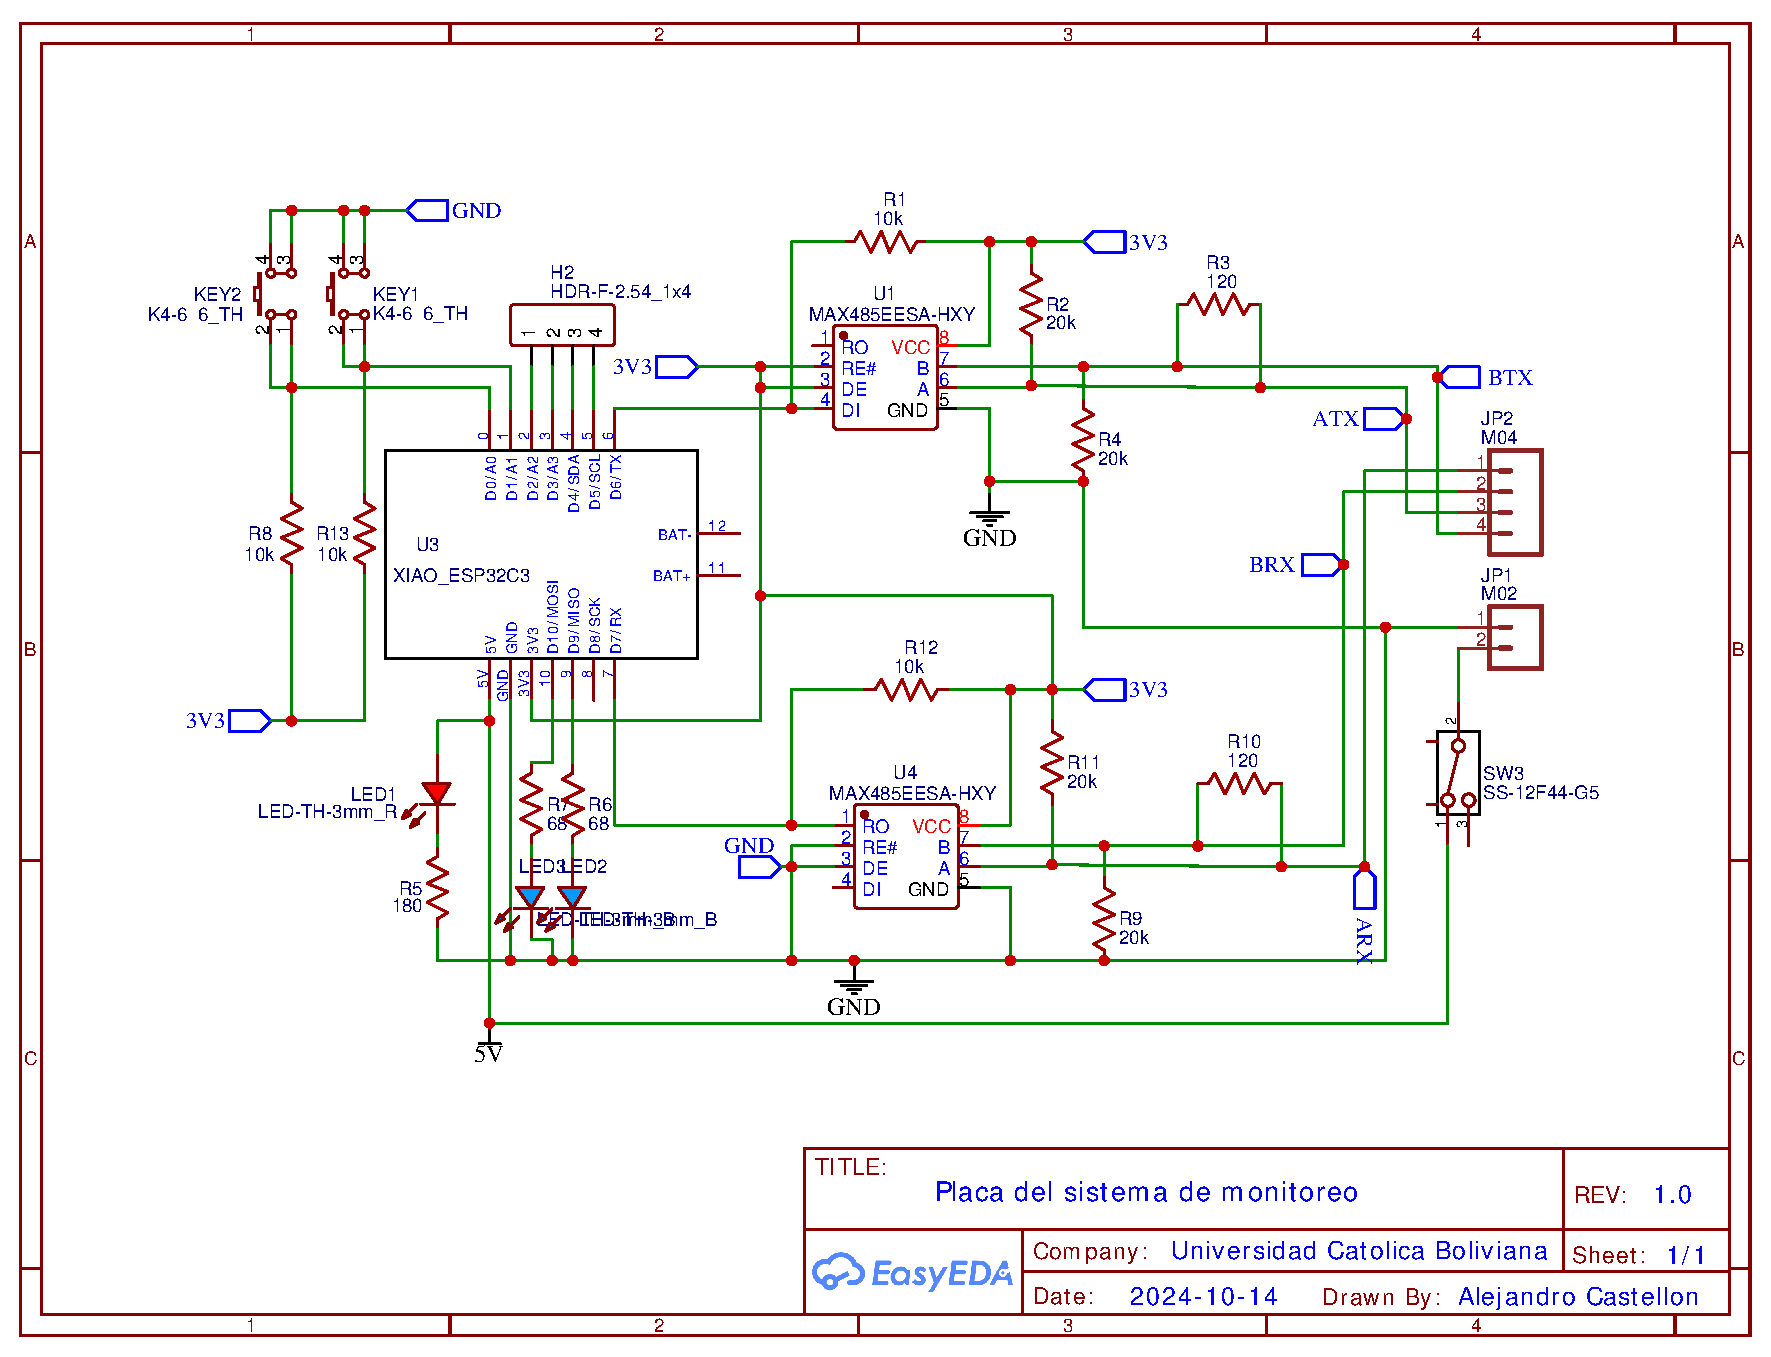
\includepdf[pages={1}]{PDFs/diagram_elec.pdf}

\apex{Diagrama de flujo}
\label{apx:3}
\begin{figure}[hpt]
    \centering
    % Título de figura
    \caption{Diagrama de flujo}
        % imagen 1
        \subfloat[Inicio]{\includegraphics[width=0.4\columnwidth]{Figuras/bloques1.png}}
        % separaciones | agregar una de las opciones entre cada par de imágenes
            \qquad      % figuras en la misma linea
            %\par        % siguiente línea
        % imagen 2
        \subfloat[Bucle]{\includegraphics[width=0.4\columnwidth]{Figuras/bloques2.png}}\\
    \centering{\textbf{Fuente:} Elaboración propia (2024)}
    \label{fig:flujo}
\end{figure}

\apex{Planos mecánicos}
\label{apx:4}
\includepdf[pages={1}]{PDFs/Plano1.PDF}
\includepdf[pages={1}]{PDFs/Plano2.PDF}
\includepdf[pages={1}]{PDFs/Plano3.PDF}

%Caso usted quisiera adicionar pequeñas líneas de código tal cual fueron introducidas por su persona, puede utilizar el formato a continuación.

%\begin{lstlisting}[frame=single]
  % suma de los elementos de un vector
 % z = 0;
 % n = length(v);
  %for i=1:1:n
  %  z = z + v[i];
 % end
%\end{lstlisting}


    
\end{document}